% This LaTeX document needs to be compiled with XeLaTeX.
\documentclass[
  10
]{article}
\usepackage[margin=2cm,includehead=true,includefoot=true,centering,]{geometry}
\usepackage{xcolor}
\usepackage{ucharclasses}
\usepackage{hyperref}
\usepackage{amsmath,amssymb}
\usepackage{amsfonts}
\usepackage[version=4]{mhchem}
\usepackage{stmaryrd}
\usepackage{bbold}
\usepackage{polyglossia}
\usepackage{fontspec}
\usepackage{ctex}
\usepackage[export]{adjustbox}
\usepackage{tabularx}
\usepackage{booktabs}

\usepackage{setspace}
\setstretch{1.2}

\makeatletter
\@ifundefined{KOMAClassName}{% if non-KOMA class
  \IfFileExists{parskip.sty}{%
    \usepackage{parskip}
  }{% else
    \setlength{\parindent}{0pt}
    \setlength{\parskip}{6pt plus 2pt minus 1pt}}
}{% if KOMA class
  \KOMAoptions{parskip=half}}
\makeatother
\usepackage{longtable,booktabs,array}
\newcounter{none} % for unnumbered tables
\usepackage{multirow}
\usepackage{calc} % for calculating minipage widths
% Correct order of tables after \paragraph or \subparagraph
\usepackage{etoolbox}
\makeatletter
\patchcmd\longtable{\par}{\if@noskipsec\mbox{}\fi\par}{}{}
\makeatother
% Allow footnotes in longtable head/foot
\IfFileExists{footnotehyper.sty}{\usepackage{footnotehyper}}{\usepackage{footnote}}
\makesavenoteenv{longtable}
\usepackage{graphicx}
\makeatletter
\newsavebox\pandoc@box
\newcommand*\pandocbounded[1]{% scales image to fit in text height/width
  \sbox\pandoc@box{#1}%
  \Gscale@div\@tempa{\textheight}{\dimexpr\ht\pandoc@box+\dp\pandoc@box\relax}%
  \Gscale@div\@tempb{\linewidth}{\wd\pandoc@box}%
  \ifdim\@tempb\p@<\@tempa\p@\let\@tempa\@tempb\fi% select the smaller of both
  \ifdim\@tempa\p@<\p@\scalebox{\@tempa}{\usebox\pandoc@box}%
  \else\usebox{\pandoc@box}%
  \fi%
}
% Set default figure placement to htbp
\def\fps@figure{htbp}
\makeatother
\setlength{\emergencystretch}{3em} % prevent overfull lines
\providecommand{\tightlist}{%
  \setlength{\itemsep}{0pt}\setlength{\parskip}{0pt}}


\hypersetup{colorlinks=true, linkcolor=blue, filecolor=magenta, urlcolor=cyan,}
\urlstyle{same}

\usepackage{colortbl}
\definecolor{table-row-color}{HTML}{999999}
\definecolor{table-rule-color}{HTML}{999999}
%\arrayrulecolor{black!40}
\arrayrulecolor{table-rule-color}     % color of \toprule, \midrule, \bottomrule
\setlength{\aboverulesep}{0pt}
\setlength{\belowrulesep}{0pt}


\setotherlanguages{english}
\IfFontExistsTF{Source Han Serif CN}
{\newfontfamily\chinesefont{Source Han Serif CN}}
{\IfFontExistsTF{Noto Serif CJK SC}
  {\newfontfamily\chinesefont{Noto Serif CJK SC}}
  {\IfFontExistsTF{SimSun}
    {\newfontfamily\chinesefont{SimSun}}
    {\IfFontExistsTF{FangSong}
      {\newfontfamily\chinesefont{FangSong}}
      {\newfontfamily\chinesefont{Arial Unicode MS}}
}}}
\IfFontExistsTF{Times New Roman}
{\newfontfamily\englishfont{Times New Roman}}
{\IfFontExistsTF{Liberation Serif}
  {\newfontfamily\englishfont{Liberation Serif}}
  {\IfFontExistsTF{DejaVu Serif}
    {\newfontfamily\englishfont{DejaVu Serif}}
    {\newfontfamily\englishfont{Arial}}
}}


\author{}
\date{}

\begin{document}


\section{Scalable Implementation of Polynomial Filtering for Density
Functional Theory Calculation in
PARSEC}\label{scalable-implementation-of-polynomial-filtering-for-density-functional-theory-calculation-in-parsec}

Kai-Hsin Liou1 Chao Yang2 James R. Chelikowsky3

Keywords: parallel algorithm; electronic structure; density functional
theory; eigenvalue problem; polynomial filtering; spectrum slicing

\section{1. Introduction}\label{introduction}

First-principle calculations and simulations have emerged as a third
scientific tool on par with experiment and theory. Since the seminal
work of Hohenberg and Kohn in establishing the foundation (proving the
existence of a unique functional that gives the lowest value when a
system is at its ground state) of density functional theory (DFT)
{[}1{]}, and the creation of a practical calculation scheme (on finding
the ground-state energy and corresponding electronic charge density) by
Kohn and Sham {[}2{]}, DFT has become an indispensable tool for
understanding and predicting material properties. The idea that the
ground-state energy is a functional of the electronic charge density
leads to a great simplification of the corresponding many-body
Schrödinger equation. The minimization of the functional results in the
Kohn--Sham equations {[}2{]}.

The ``routinely solvable'' system size for materials has increased from
dozens of atoms in the 1990s to thousands of atoms nowadays, thanks to
theoretical developments and advances in computing power. Real-space
pseudopotential DFT along with the Chebyshev-filtered subspace iteration
(CheFSI) algorithm has shown the ability to solve the electronic
structures of systems containing up to 20,000 atoms (e.g., a silicon
nanocrystal, Si20389H3076 {[}3{]}) {[}4, 5{]}.

The bottleneck of DFT calculation often rests on an eigensolver.
However, it is now widely recognized that during a self-consistent-field
(SCF) calculation, the linear eigenvalue problems do not need to be
solved to full accuracy in the early SCF iterations when the electronic
charge density is far from converged {[}6{]}. The CheFSI algorithm
exploits this characteristic of SCF calculations and focuses on
improving the wave functions and electronic charge density at the same
time over SCF iterations. This strategy often proves to be time-saving
when solving the nonlinear eigenvalue problem defined by the Kohn--Sham
equations.

The CheFSI algorithm has been adopted in several other large-scale DFT
based electronic structure analysis software such as DGDFT {[}7{]},
SPARC {[}8{]}, and FE-DFT {[}9{]}. A library that implements a Chebyshev
Accelerated Subspace Iteration has recently become available {[}10{]}.
In 2016 Michaud-Rioux et al.~also demonstrated that a combination of
CheFSI and their partial Rayleigh--Ritz method enables the routine
calculation of thousands of atoms with only moderate computational
resources {[}11{]}. The CheFSI algorithm is applied by Banerjee et
al.~{[}12{]} to not only the original Kohn--Sham Hamiltonian, but also
the projected subspace problem. It is even employed in introductory
textbooks {[}13{]}.

Here, we use PARSEC, a DFT software package featuring real-space
calculations and the pseudopotential approximation, to solve the
Kohn--Sham equations {[}14{]}. The real-space representation of the wave
functions has the advantages of making a parallel implementation and
software development relatively straightforward {[}4{]}. Furthermore,
pseudopotential theory and techniques encapsulate the chemically inert
core electrons into the ion core and consider them as part of the
external electric field felt by valence electrons. This enables us to
solve the Kohn--Sham equations only for the valence electrons, greatly
reducing the computational demands.

CheFSI has proven to be an effective way for approximating the invariant
subspace associated with the occupied states in a real-space DFT
calculation algorithm. The advantages of using Chebyshev polynomial
filtering are: 1) It only requires multiplying the Hamiltonian matrix,
H, with vectors; 2) The three-term recurrence of the Chebyshev
polynomials makes the filtering process efficient in terms of memory
footprint; 3) Ritz vectors from a previous SCF iteration can be used as
the starting guess for the desired eigenvectors in the current SCF
iteration; 4) CheFSI is a block method that increases concurrency and
memory efficiency.

For small to medium sized problems, the time cost of CheFSI is dominated
by the multiplication of H with vectors. These operations can be
efficiently parallelized. However, for large systems the Rayleigh--Ritz
procedure used to extract the desired eigenvalue approximation and the
other dense linear algebra operations required to construct and analyze
the projected problem become a bottleneck. Spectrum slicing (SS) methods
have been proposed to address this issue. Spectrum slicing refers to
dividing the spectrum of interest into several spectral slices and
computing approximate eigenpairs within each slice simultaneously.
Although the SS methods can clearly reduce the overhead associated with
solving the projected subspace problem (because each slice contains a
much smaller subset of the eigenvalues), it needs to compute interior
eigenvalues that may be clustered. A different type of polynomial
filters needs to be constructed to amplify eigenvalues within each
slice, just as a Chebyshev polynomial is used to amplify eigenvalues at
the left end of the spectrum in the CheFSI method. The degree of these
types of polynomials, which we will refer to as ``bandpass filter
polynomials,'' may be much higher than that of the Chebyshev polynomials
used in CheFSI when the eigenvalues to be computed are very close to
each other.

Previously, a thick-restart Lanczos algorithm was proposed to compute
interior eigenvalues filtered by bandpass filter polynomials {[}15{]}.
The method converges fast, but has limited levels of concurrency. In
this paper, we propose using a subspace iteration method to compute
interior eigenpairs. Although the subspace iteration method tends to
have a slower convergence rate, especially at the beginning of a SCF
calculation when no good initial guess to the approximate eigenpairs is
available, it is a block method that exhibits multiple levels of
concurrency that lead to superior parallel scalability.

To address the potential slow convergence of the subspace iteration
method, we propose using CheFSI in the first few SCF iterations and then
transitioning to SS based polynomial filtering in the subsequent SCF
iterations. We show by numerical examples that this hybrid polynomial
filtering scheme is effective.

One of the keys to achieving scalable performance in SS is an optimal
partition of the desired part of a spectrum. The partition must take
into account the distribution of eigenvalues (which can be obtained from
either an estimated density of states or approximated eigenvalues
computed in a previous SCF iteration) as well as load balance needs in a
parallel implementation. We present a practical way to perform such a
partitioning.

In Section 2, we briefly review the governing equations of Kohn--Sham
DFT eigenvalue problems. We describe how to perform polynomial filtering
in Section 3. In particular, we review the major computational
components of both CheFSI and SS algorithms. We discuss how to construct
both Cheybshev and bandpass filter polynomials for computing eigenpairs
at the low end and within a spectral slice respectively. Furthermore, we
examine how to partition the spectrum into spectral slices using an
estimated density of states obtained from a Lanczos iteration, and
refine the partition using Ritz values obtained from previous SCF
iterations. In Section 4, we discuss a number of issues related to an
efficient implementation of polynomial filtering algorithms. These
include the use of an appropriate data layout for carrying out the
computation on a two-dimensional (2D) process grid, how to achieve good
load balance, and the type of communications involved in the parallel
implementation. We present a number of computational examples in Section
5. In particular, we show the performance characteristics of both CheFSI
and SS, and note the relative cost of Hamiltonian vector multiplications
and dense matrix computations performed within a subspace. We
demonstrate that rapid SCF convergence can be achieved in a hybrid
CheFSI and SS scheme when the degrees of bandpass filters used in SS are
sufficiently high for a number of test problems. These results indicate
that the use of subspace iteration and bandpass filters can produce
sufficiently accurate approximations to the desired eigenpairs. We
demonstrate that SS has much better strong parallel scalability compared
with CheFSI for a sufficiently large problem when it is performed on an
adequately large number of compute cores. In fact, for a large test
problem, we show the crossover point (in terms of computational
resources) beyond which the time cost used by SS is lower than that used
by CheFSI.

\section{2. Kohn--Sham Equations}\label{kohnsham-equations}

The Kohn--Sham equations are used to reformulate a quantum many-body
problem of electrons in molecules and solids in terms of a system of
single-particle equations (in atomic units) of the form

\[
\left[ - \frac {1}{2} \nabla^ {2} + V _ {\text {ion}} (\mathbf {r}) + V _ {\mathrm{H}} [ n (\mathbf {r}) ] + V _ {\mathrm{xc}} [ n (\mathbf {r}) ] \right] \psi_ {i} (\mathbf {r}) = \varepsilon_ {i} \psi_ {i} (\mathbf {r}), \tag {1}
\]

where \(V _ { \mathrm { i o n } }\) is the external ionic potential
experienced by an electron, \(V _ { \mathrm { H } }\) the Hartree
potential that describes electron repulsion, and
\(V _ { \mathrm { x c } }\) the exchange-correlation potential that
accounts for manybody effects. The single-particle orbital
\(\psi _ { i }\) and the corresponding energy \(\varepsilon _ { i }\)
form the ith eigenpair of the Kohn--Sham Hamiltonian
\(\begin{array} { r } { H _ { \mathrm { K S } } = - \frac { 1 } { 2 } \nabla ^ { 2 } + V _ { \mathrm { i o n } } ( \mathbf { r } ) + V _ { \mathrm { H } } [ n ( \mathbf { r } ) ] + V _ { \mathrm { x c } } [ n ( \mathbf { r } ) ] } \end{array}\)
, which is a functional of the ground-state electronic charge density
\(n ( \mathbf { r } )\) defined by

\[
n (\mathbf {r}) = 2 \sum_ {i = 1} ^ {N _ {s}} f _ {i} | \psi_ {i} (\mathbf {r}) | ^ {2}, \tag {2}
\]

where the prefactor \(2\) accounts for electronic spins (which we do not
distinguish in this work), \(N _ { s }\) is the number of states being
calculated, and \(f _ { i }\) is the Fermi--Dirac distribution function:

\[
f (t) = \frac {1}{\exp ((t - \varepsilon_ {\mathrm{F}}) / k _ {B} T) + 1} \tag {3}
\]

evaluated at the single-particle energy \(\varepsilon _ { i } .\) .
Here, \(k _ { \mathrm { B } }\) is the Boltzmann constant, and \(T\) is
the temperature, which is typically set to 80 K through our simulations.
This issues proper occupancy for nearly degenerate states. The
eigenvalues \(\varepsilon _ { i } \mathrm { { ^ { s } } }\) are ordered
in ascending order,
\(i . e . , \varepsilon _ { 1 } \leq \varepsilon _ { 2 } \leq \cdot \cdot \cdot\)
. The first \(N _ { \mathrm { o c c } }\) eigenpairs,
\(( \psi _ { i } , \varepsilon _ { i } ) , i = 1 , 2 , . . . , N _ { \mathrm { o c c } }\)
, where \(N _ { \mathrm { o c c } }\) is the number of occupied states,
are known as the occupied states, and all others are known as the
unoccupied states. We assume spin unpolarized states.

If there is a spectral gap between the occupied and unoccupied states,
the Fermi level \(\varepsilon _ { \mathrm { F } }\) is between
\(\varepsilon _ { N _ { \mathrm { o c c } } }\) and
\(\varepsilon N _ { \mathrm { o c c } }\) and ensures the electronic
charge density \(n ( \mathbf { r } )\) integrates to
\(2 N _ { \mathrm { o c c } }\) . When the temperature \(T\) is
relatively low, \(f ( t )\) decreases from 1 to 0 rapidly near the Fermi
level. As a result, the number of effective terms \(N _ { s }\) to be
summed in (2) is slightly larger than the number of occupied states. For
metallic systems no gap occurs between the occupied and unoccupied
states. For finite systems, a vanishingly small gap might occur. A
larger \(T\) may be needed to ensure that the Kohn--Sham problem is well
posed by allowing the admixtures of states near the Fermi level. In this
case, \(N _ { s }\) may be much larger than
\(N _ { \mathrm { o c c } } , \ i . e .\) , more states are included in
the summation in (2) to make sure the system is neutral.

The Kohn--Sham equations define a nonlinear eigenvalue problem. The
Hamiltonian depends on the electronic charge density, which is in turn
defined in terms of the eigenpairs of the Hamiltonian. In practice, the
solution to (1) is computed iteratively by solving a sequence of linear
eigenvalue problems defined by a sequence of electronic charge densities
\(n ^ { ( i ) } \mathrm { { _ S } }\) that become self-consistent at
convergence, \(i . e . ,\) the electronic charge density
\(n ^ { ( i ) }\) obtained from the eigenvectors of
\(H _ { \mathrm { K S } } ( n ^ { ( i - 1 ) } )\) ) is the same, or
within some predefined tolerance, as \(n ^ { ( i - 1 ) }\) for some
\(i .\)

When \(H _ { \mathrm { K S } }\) is discretized by a real-space method
such as finite difference, the discretized \(H _ { \mathrm { K S } }\)
is extremely sparse. The dimension of the discretized Hamiltonian is
much larger than the number of eigenstates \(N _ { s }\) to be computed.
Therefore, an iterative method is preferred to compute the desired
eigenstates.

\section{3. Polynomial Filtering}\label{polynomial-filtering}

There are a number of iterative methods for solving large sparse
eigenvalue problems. In the early days, PARSEC first used the implicitly
restarted Lanczos (IRL) algorithm implemented in the ARPACK software
{[}16, 14{]}. Although the method is robust and accurate, its
computational cost increases rapidly with respect to the number of
eigenstates that need to be computed. This is partly due to the fact
that more iterations and restarts are needed to converge eigenvalues
deep inside the spectrum, \(e . g .\) , near the Fermi level. Moreover,
IRL can only make use of a good initial guess to a single eigenvector.
This feature makes it less effective for subsequent SCF iterations in
which a good initial guess to the entire subspace associated with the
occupied states is available. Furthermore, IRL is not a block method,
i.e., in IRL the Hamiltonian can be multiplied with only one vector at a
time. This makes it less scalable on a parallel machine.

Both the LOBPCG {[}17{]} and Davidson algorithms {[}18{]} are block
algorithms that can take advantage of a good initial guess of the
subspace associated with the occupied states. However, without a good
preconditioner, these methods tend to converge slowly. For real-space
methods, it is generally difficult to construct an effective
preconditioner. Thus these methods are less effective. Furthermore,
these methods are less stable when a large number of eigenpairs are to
be computed {[}19{]}.

The use of polynomial filtering for computing eigenvalues of a large
sparse matrix dates back over 50 years to the work of Stiefel {[}20{]}
and was carefully examined by Yang {[}21{]}. The innovative use of
Chebyshev filtering for solving the Kohn--Sham eigenvalue problem was
first developed by Zhou et al.~{[}22{]}, where effective spectral bounds
were developed to construct an effective Chebyshev filtering polynomial.
The CheFSI was used to compute the invariant subspace associated with
the occupied states instead of eigenvectors explicitly. The success of
Zhou et al.~brought a speed-up of five to ten times compared to other
eigensolvers, and marked the beginning of the prevalence of the CheFSI
method in electronic structure calculations.

We review the CheFSI method in Section 3.1, and briefly discuss how to
construct a bandpass polynomial filter to amplify eigencomponents
associated with interior eigenvalues in Section 3.2. We explain why it
is a good idea to combine spectrum slicing using bandpass polynomials
with CheFSI in a hybrid polynomial filtering algorithm for accelerating
the SCF iteration in Section 3.3.

\section{3.1. Chebyshev-filtered subspace
iteration}\label{chebyshev-filtered-subspace-iteration}

An mth-degree Chebyshev polynomial of the first kind can be defined
recursively as

\[
T _ {m} (t) = 2 t T _ {m - 1} (t) - T _ {m - 2} (t), \tag {4}
\]

with \(T _ { 0 } ( t ) = 1\) and \(T _ { 1 } ( t ) = t .\) . The
magnitude of \(T _ { m } ( t )\) is bounded by 1 within \([ - 1 , 1 ]\)
and grows rapidly outside of this interval. Figure 1 shows Chebyshev
polynomials of various degrees.

\pandocbounded{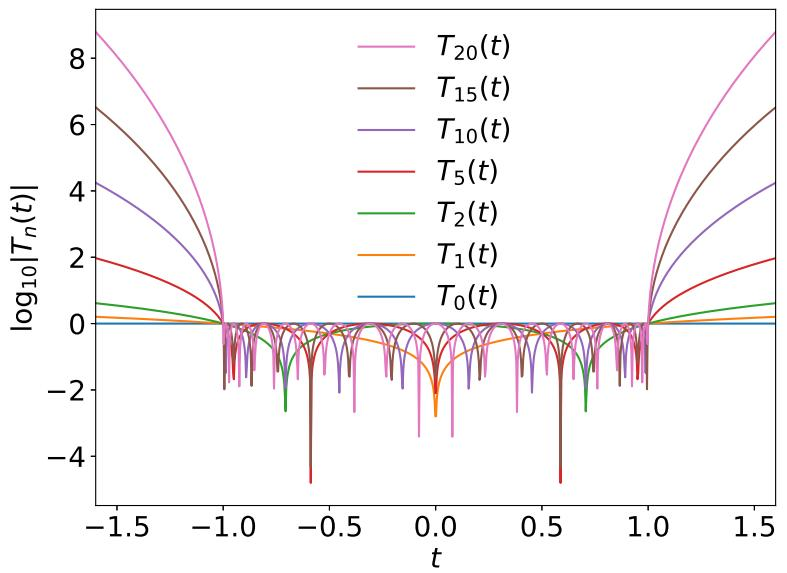
\includegraphics[keepaspectratio,alt={image}]{images/3d76d1cb330dd6db914f1392fc2e828e641b28b33538f979464d476ef2f08b4d.jpg}}

Figure 1: Chebyshev polynomials of the first kind.

We define the estimated lower and upper bounds of the spectrum of
\(H , \lambda _ { \mathrm { l b } }\) and
\(\lambda _ { \mathrm { u b } } .\) , and an estimated Fermi level, εF.
By mapping the unwanted eigenvalues (e.g., the unoccupied states) of the
Kohn--Sham Hamiltonian H enclosed by
\([ \varepsilon _ { \mathrm { F } } , \lambda _ { \mathrm { u b } } ] \mathrm { t o } [ - 1 , 1 ]\)
through the linear transformation (t − \(c ) / e\) , where
\(c = ( \varepsilon _ { \mathrm { F } } + \lambda _ { \mathrm { u b } } ) / 2\)
and
\(e = ( \lambda _ { \mathrm { u b } } - \varepsilon _ { \mathrm { F } } ) / 2 .\)
we can use
\(\hat { T } _ { m } ( H ) = T _ { m } ( ( H - c I ) / e ) \iota\) v to
amplify the eigenvector components in v that correspond to eigenvalues
outside of
\(\left[ \varepsilon _ { \mathrm { F } } , \lambda _ { \mathrm { u b } } \right]\)
{]}. Applying \(T _ { m } ( ( H - c I ) / e )\) repeatedly to a block of
vectors V filters out the eigenvectors associated with eigenvalues in
\(\left[ \varepsilon _ { \mathrm { F } } , \lambda _ { \mathrm { u b } } \right]\)
{]}. The desired eigenpairs can be obtained through the standard
Rayleigh-- Ritz procedure {[}23{]} described in Algorithm 3.

Owing to the three-term recurrence in
\(( 4 ) , W = { \hat { T } } _ { m } ( H ) V\) can be computed
recursively without forming \(\hat { T } _ { m } ( H )\) explicitly in
advance. Algorithm 1 describes how this step is carried out in detail.
To maintain numerical stability, we orthonormalize vectors in W . The
orthonormalization can be performed by a (modified) Gram--Schmidt
process or by a Householder transformation based QR factorization
{[}24{]}.

Although these algorithms can achieve high accuracy, they are not the
most efficient ones, especially when implemented on a distributed,
parallel computer. We choose the Cholesky QR algorithm described in
Algorithm 2 to perform orthonormalization because Algorithm 2 can make
use of highly efficient matrix computation kernels such as matrix-matrix
multiplication, Choleksy factorization, and triangular substitution with
multiple right-hand sides. We perform a fixed number of Chebyshev
polynomial filtering (Algorithm 1) and orthonormalization (Algorithm 2)
steps before using Rayleigh--Ritz procedure to extract approximations to
the desired eigenvalues and eigenvectors. The overall Chebyshev-filtered
subspace iteration procedure is described in Algorithm 4.

In Algorithm 1, the required inputs are
\(\lambda _ { \mathrm { l b } } , \lambda _ { \mathrm { u b } } , \varepsilon _ { \mathrm { F } } .\)
, and a filter degree, m. In the first SCF iteration,
\(\lambda _ { \mathrm { l b } }\) and \(\lambda _ { \mathrm { u b } }\)
can be calculated by running a few Lanczos iterations, and
\(\varepsilon _ { \mathrm { F } }\) is typically set to
\(( 2 \lambda _ { \mathrm { l b } } + \lambda _ { \mathrm { u b } } ) / 3\)
. In the subsequent SCF iterations, \(\lambda _ { \mathrm { l b } }\)
can be replaced by the lowest Ritz value while εF can be computed by
solving an equation of the conservation of valence electrons,
\(\begin{array} { r } { i . e . , N _ { \mathrm { e } } = \int n ( \mathbf { r } ) \mathrm { d } \mathbf { r } } \end{array}\)
, where \(N _ { \mathrm { e } }\) is the total number of valence
electrons. See the work of Saad {[}25{]} and Zhou et al.~{[}5{]} for
more details on Chebyshev filtering.

We note that for systems with a relatively large gap between the
occupied and unoccupied states (e.g., insulators), it may not be
necessary to perform the Rayleigh--Ritz procedure because the basis
vectors \(\psi _ { i } \mathrm { ^ s }\) used in (2) can be any
orthonormal basis vectors that span the same invariant subspace defined
by the occupied states. For gapless systems (metals) or systems with a
relatively small energy gap, approximate eigenvalues near the gap are
needed to obtain the occupancy defined in (3). Moreover, the use of the
Rayleigh--Ritz procedure may also allow us to lock eigenvectors that
have already converged to reduce the computational cost of subsequent
subspace iterations.

Algorithm 1 Chebyshev filtering

1: procedure
\(W = \text{CHEBYFILTER}(H, V, m, \varepsilon_{\text{F}}, \lambda_{\text{ub}}, \lambda_{\text{lb}})\)
2: \(e = (\lambda_{\text{ub}} - \varepsilon_{\text{F}})/2\) 3:
\(c = (\lambda_{\text{ub}} + \varepsilon_{\text{F}})/2\) 4:
\(\sigma = e/(c - \lambda_{\text{lb}})\) 5: \(\tau = 2/\sigma\) 6:
\(W = (HV - cV)(\sigma/e)\) 7: for \(i = 2 \rightarrow m\) do 8:
\(\sigma_{new} = 1/(\tau - \sigma)\) 9:
\(W_t = (HV - cV)(2\sigma_{\text{new}}/e) - (\sigma\sigma_{\text{new}})V\)
10: V = W 11: \(W = W_t\) 12: \(\sigma = \sigma_{new}\)

Algorithm 2 Cholesky QR

1: procedure \(V = \text{ORTH}(W)\) 2: \(A = W^{T}W\) ▷ A is positive
definite 3: Find an upper triangular R such that \(A = R^{T}R\) ▷
Cholesky factorization 4: \(V = WR^{-1}\)

Algorithm 3 Rayleigh--Ritz procedure

1: procedure \((V,D)=\text{RAYLEIGHRITZ}(H,V)\) 2: \(A=V^{T}HV\) 3:
Compute Q and D such that AQ=QD and \(Q^{T}Q=I.\) \(\triangleright D\)
has the Ritz values 4: V=VQ

\section{3.2. Spectrum slicing}\label{spectrum-slicing}

When the number of eigenpairs to be computed (usually the occupied
states plus some unoccupied states), \(N _ { s } ,\) is relatively small
\(( e . g .\) , less than a thousand), the computational cost of CheFSI
is dominated by sparse matrix-vector multiplications HV . By making
these multiplications scalable through the distribution of vectors in V
on a 2D process grid, we can compute the desired eigenpairs efficiently.
However, as the system size increases, the number of eigenpairs
\(N _ { s }\) becomes very large. As a result, orthonormalization and
Rayleigh--Ritz procedure, which scale cubically with respect to
\(N _ { s }\) , start to dominate the computational cost. Furthermore,
because these types of computation involve more collective communication
among all processes, the overall computation is difficult to scale to a
large number of compute cores.

Algorithm 4 Chebyshev-filtered subspace iteration

1: procedure
\((V,D)=\text{CHEBYSUBIT}(H,V,m,\varepsilon_{\mathrm{F}},\lambda_{\mathrm{ub}},\lambda_{\mathrm{lb}},\text{maxiter})\)
2: for iter = 1 → maxiter do 3: W = ChebyFilter(H, V, m,
\(\varepsilon_{F}\) , \(\lambda_{ub}\) , \(\lambda_{lb}\) ); 4: V =
Orth(W); 5: \((V,D)=\text{RayleighRitz}(H,V)\) ;

To address this difficulty, a spectrum slicing algorithm was proposed by
Schofield et al.~{[}26{]} to divide the eigenvalues to be computed into
several subintervals (i.e., slices) that can be examined simultaneously.
Eigenvalues within each subinterval can still be computed by a
polynomial filtered iterative method. However, with the exception of the
leftmost subinterval, a different type of filter needs to be constructed
to focus on eigenvalues within the other subintervals.

Schofield et al.~{[}26{]} and Li et al.~{[}15{]} implemented methods for
constructing polynomial filters \(p _ { m } ( t )\) for computing
eigenvalues within an interval {[}a, b{]}. A thick-restart Lanczos
iteration is used to compute the largest eigenpairs of
\(p _ { m } ( H )\) . Although these studies examined several key issues
of the SS algorithm, and provided a proof of concept, a few important
details such as how to partition the spectrum to achieve scalable
performance on a large number of compute cores were not addressed.

Here we examine several implementation details that are key to achieving
scalable performance. Instead of using a thick-restarted Lanczos
iteration method, which cannot take full advantage of a 2D process grid
to compute eigenpairs within each interval, we propose to use a subspace
iteration method to compute the largest eigenpairs of
\(p _ { m } ( H )\) . However, because the subspace iteration method
typically has a slower convergence rate, a high degree polynomial or a
large number of iterations may be required.

\section{3.2.1. Spectrum partition}\label{spectrum-partition}

Although spectrum slicing is conceptually easy to understand, there are
a number of issues that we must address in order to make it a practical
computational method. The first pertains to the partition of a spectrum
into distinct slices that can be examined in parallel. Because we often
do not know how the eigenvalues are distributed in advance of the
solution, this is not a trivial task.

One way to estimate the distribution of eigenvalues is to use the
Lanczos algorithm {[}27{]}. We use an ensemble of
\texttt{randomly\ generated\ vectors\ \$\textbackslash{}begin\{array\}\ \{\ r\ \}\ \{\ v\ \^{}\ \{\ (\ j\ )\ \}\ ,\ j\ =\ 1\ ,\ 2\ ,\ \textbackslash{}ldots\ \textbackslash{}ell\ ,\ \}\ \textbackslash{}end\{array\}\$\ ,\ with\ Gaussian\ independent\ and\ identically\ distributed\ elements\ to\ start}
k-step Lanczos iterations, which produce \(\ell \ k \times k\)
tridiagonal matrices \(T ^ { ( j ) } , j = 1 , 2 , . . . , \ell\) . If
the eigenvalues of \(T ^ { ( j ) }\) are denoted by
\(\theta _ { i } ^ { ( j ) } , i = 1 , 2 , . . . , k\) , and the first
component of the eigenvector associated with
\(\theta _ { i } ^ { ( j ) }\) is denoted by
\(\tau _ { i } ^ { ( j ) }\) i, an approximation to the density of
states can be expressed as

\[
d (t) = \sum_ {j = 1} ^ {\ell} \sum_ {i = 1} ^ {k} (\tau_ {i} ^ {(j)}) ^ {2} \exp \left(- \frac {(t - \theta_ {i} ^ {(j)}) ^ {2}}{\sigma_ {i} ^ {(j)}}\right), \tag {5}
\]

where
\(\sigma _ { i } ^ { \left( j \right) } \mathrm { \overline { { s } } }\)
are scaling parameters that should be chosen carefully {[}27{]}. Note
that the ` Lanczos runs can be carried out in parallel on different
process groups.

Although the function d(t) describes the distribution of eigenvalues,
the value d(t) for a specific t is not so useful. It is more useful to
work with the cumulative density of states defined as

\[
g (t) \equiv \int_ {- \infty} ^ {t} d (s) \mathrm{d} s = \frac {\sqrt {\pi}}{2} \sum_ {j = 1} ^ {\ell} \sum_ {i = 1} ^ {k} (\tau_ {i} ^ {(j)}) ^ {2} \sigma_ {i} ^ {(j)} \left[ \operatorname{erf} \left(\frac {t - \theta_ {i} ^ {(j)}}{\sigma_ {i}}\right) + 1 \right]. \tag {6}
\]

In particular, given two real numbers \(t _ { 1 }\) and \(t _ { 2 }\)
with \(t _ { 1 } < t _ { 2 } , g ( t _ { 2 } ) - g ( t _ { 1 } )\)
yields the number of eigenvalues within the interval
\([ t _ { 1 } , t _ { 2 } )\) .

The strategy we use to partition the spectrum of interest is to divide
the interval {[}a, b{]}, where a is a lower bound of the eigenvalues of
H and b is an (estimated) upper bound of the occupied states, uniformly
into p slices of equal size
\([ l _ { i } , u _ { i } ) , i = 1 , 2 , . . . , p .\) , where
\(l _ { 1 } = a , u _ { p } = b\) and \(l _ { i } = u _ { i - 1 }\) for
\(i > 1 , u _ { i } = l _ { i + 1 }\) for \(i < p .\) . We call this
partition scheme a uniform partition. The optimal number of slices \(p\)
depends on a number of factors, which we will discuss later in Section
4.2. The uniform partition will also need to be modified to achieve good
load balance in a parallel implementation.

In order to avoid missing eigenpairs in each slice
\([ l _ { i } , u _ { i } )\) , we construct the polynomial on a
slightly larger interval \([ l _ { i } - \delta , u _ { i } + \delta ]\)
, where δ is typically chosen to be a fraction of the width of a slice.
(We use \(\delta = ( u _ { i } - l _ { i } ) / 1 0\) in our
simulations.)

We use
\(c _ { i } = g ( u _ { i } + \delta ) - g ( l _ { i } - \delta )\) to
estimate the number of eigenvalues within that augmented interval. Note
that some of the eigenvalues within
\([ l _ { i } - \delta , u _ { i } + \delta )\) overlap with those in
\([ l _ { i - 1 } - \delta , u _ { i - 1 } +\) δ) and
\([ l _ { i + 1 } - \delta , u _ { i + 1 } + \delta )\) , as shown in
Figure 2. Once the eigenvalues in each slice are computed, we use the
slice bounds \(l _ { i }\) and \(u _ { i }\) to select eigenvalues and
eigenvectors to be included in the occupancy and electronic charge
density calculation. An eigenvalue in the overlap regions is possibly
captured by both adjacent slices, but will be counted by only one of the
two adjacent slices when the SCF calculation approaches convergence. The
overlaps between adjacent augmented slices allow us to eliminate the
need to orthogonalize approximate eigenvectors computed in different
slices, which requires additional data communication.

\pandocbounded{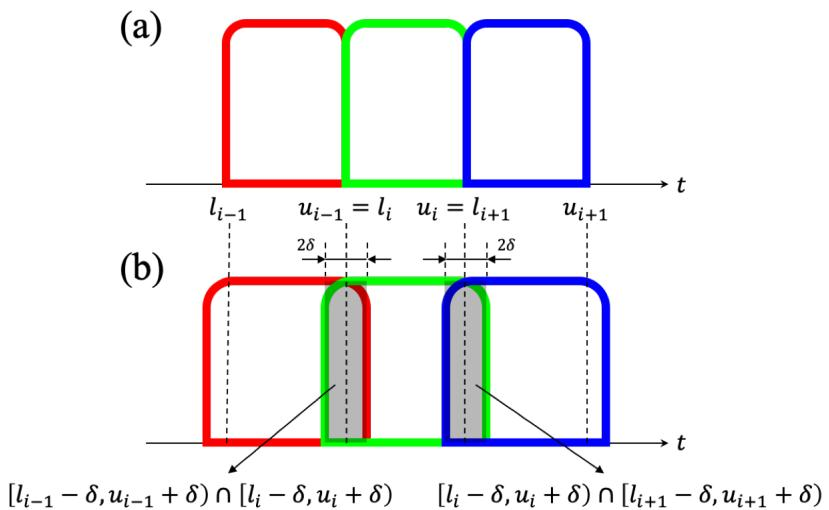
\includegraphics[keepaspectratio,alt={image}]{images/06caa5be0ee022b0f970b317b80a7527419af73083ffc83be89d2587471d13c2.jpg}}

Figure 2: (a) An illustration of uniform partitioning. (b) Extension of
the bounds of a filter by δ in both directions, and overlaps (shaded
regions) of 2δ between adjacent slices.

Based on the eigenvalue count \(c _ { i }\) and the degree of the
bandpass filter used to amplify eigenvalues within the ith slice, we
assign an appropriate number of processes to each slice to balance the
computational load among different processes. We will discuss the load
balance details in Section 4.2.

An alternative way to partition a spectrum is to determine values
\(l _ { i }\) and \(u _ { i }\) such that
\(g ( u _ { i } ) - g ( l _ { i } )\) are approximately the same for all
\(i \mathrm { \ ' } _ { \mathrm { S } }\) . This approach will yield
slices of different spectral widths even though each slice contains
nearly the same number of eigenvalues. The potential difficulty with
this approach is that bandpass filters of drastically different degrees
may be needed for different slices (see the next section), thereby
making load balancing more difficult to achieve.

We should point out that the use of the Lanczos-based density of states
estimation to partition the spectrum is only needed in the first few SCF
iterations. When the Ritz values computed from each spectral slice are
sufficiently accurate, we can use them to refine the spectrum partition.
Such a partition will not change much in subsequent SCF iterations.

\section{3.2.2. Filter polynomial
construction}\label{filter-polynomial-construction}

The bandpass filter polynomials we construct can have a large impact on
the convergence of the SS algorithm. An ideal filter \(F ( t )\) should
map the eigenvalues within a spectral slice \([ l , u ]\) to a much
larger value than the values of F outside of this interval (but within
\([ \lambda _ { \operatorname* { m i n } } , \lambda _ { \operatorname* { m a x } } ]\)
. If the interval {[}l, u{]} is sufficiently large, the bandpass filters
proposed by Schofield et al.~{[}26{]} generally works well. These
bandpass filter functions are expanded in terms of Chebyshev
polynomials. To simplify the discussion, let us assume the eigenvalues
of H are within \([ - 1 , 1 ]\) , and we are interested in the
eigenvalues within an interval \([ l , u ]\) with \(- 1 < l < u < 1\) .
With
\(\begin{array} { r } { \alpha _ { k } = \frac { \pi } { k + 2 } } \end{array}\)
, the following polynomial filter

\[
F (t) \approx p (t) = \sum_ {i = 0} ^ {k} \gamma_ {i} g _ {i} ^ {k} T _ {i} (t), \tag {7}
\]

where

\[
\gamma_ {i} = \left\{ \begin{array}{l l} \frac {1}{\pi} (\cos^ {- 1} (l) - \cos^ {- 1} (u)) & \text { as } i = 0, \\ \frac {2}{\pi} (\frac {\sin (i \cos^ {- 1} (l)) - \sin (i \cos^ {- 1} (u))}{i}) & \text { as } i > 0, \end{array} \right. \tag {8}
\]

and

\[
g _ {i} ^ {k} = \frac {\left(1 - \frac {i}{k + 2}\right) \sin (\alpha_ {k}) \cos (i \alpha_ {k}) + \frac {1}{k + 2} \cos (\alpha_ {k}) \sin (i \alpha_ {k})}{\sin (\alpha_ {k})}, \tag {9}
\]

amplifies \(\lambda \in ( l , u )\) .

Figure 3 shows four bandpass filters of different degrees defined on the
interval \([ - 0 . 8 , - 0 . 7 ]\) . Note that in practice we will use
\(l _ { i } - \delta\) and \(u _ { i } + \delta\) as bounds in
polynomial filtering but select the converged eigenpairs based on
\(l _ { i }\) and \(u _ { i }\) , as explained in Section 3.2.1.

\pandocbounded{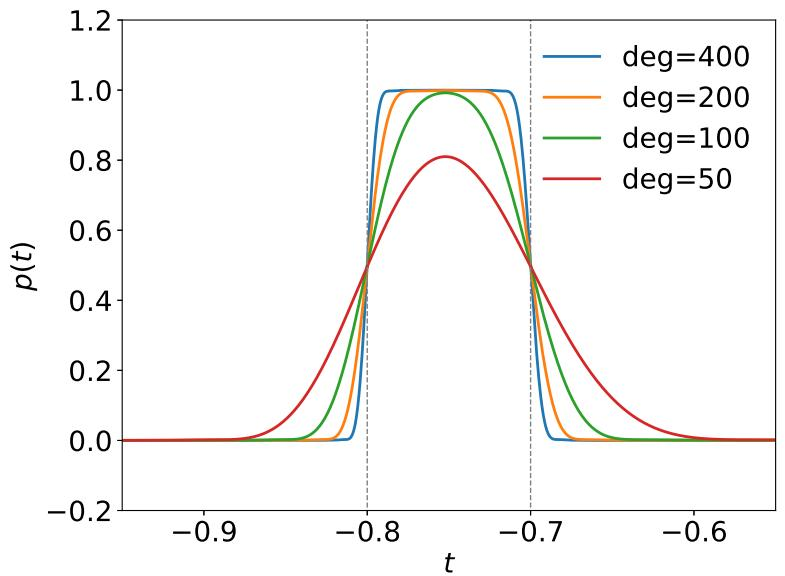
\includegraphics[keepaspectratio,alt={image}]{images/1ebd1a51d2c2f0b80e887bd7e49b543ec1df8fda7bde128c084389cfaed021e1.jpg}}

Figure 3: Bandpass polynomial filters of different degrees. The dashed
lines indicate the lower and upper bounds of the slice.

If {[}l, u{]} is relatively small compared with the spectrum width of
\(H ,\) a polynomial filter constructed from a least squares
approximation to the Dirac-δ distribution (function), which was proposed
by Li et al.~{[}15{]}, works well. Such a polynomial can be expressed as

\[
F _ {k} (t) = \sum_ {j = 0} ^ {k} \mu_ {j} T _ {j} (t), \tag {10}
\]

with

\[
\mu_ {j} = \left\{ \begin{array}{l l} \frac {1}{2} & \text { as   } j = 0, \\ \cos (j \cos^ {- 1} (\gamma)) & \text { otherwise }, \end{array} \right. \tag {11}
\]

where \(\gamma\) is the center of the Dirac-δ function. By specifying
the value of \(F ( t )\) at the bounds, we can determine the degree of
the polynomial.

We should note that a Chebyshev polynomial can be used as the filter for
the leftmost slice. Because the degree of the Chebyshev polynomial
required to amplify the eigenvalues in the leftmost slice is typically
much lower than those of the polynomials constructed for other interior
slices, we may include more eigenvalues in the leftmost slice in a
parallel implementation of the SS algorithm to achieve good load
balance. We will discuss this more in Section 4.2.

\section{3.2.3. Lanczos vs subspace
iteration}\label{lanczos-vs-subspace-iteration}

In the previous work by Schofield et al.~{[}26{]} and Li et
al.~{[}15{]}, polynomial filtering is combined with a thick-restarted
Lanczos algorithm to generate a Krylov subspace of the form

\[
\mathcal {K} (F (H), v _ {0}) = \{v _ {0}, F (H) v _ {0}, F ^ {2} (H) v _ {0}, \dots \}, \tag {12}
\]

where \(v _ { 0 }\) is typically chosen to be a random starting vector.
Rayleigh--Ritz procedure is then performed on the orthonormal basis V of
\(\mathcal { K } ( F ( H ) , v _ { 0 } )\) produced by the Lanczos
algorithm. Because the eigenpairs of interest are those associated with
the largest eigenvalues of \(F ( H )\) , which are known to emerge
rapidly {[}28{]}, this approach can produce highly accurate
approximations after k iterations, where k is typically a small (e.g., 2
to 3) multiple of the number of eigenvalues within the the interval of
interest. This observation was reported by Schofield et al.~{[}26{]}.
However, the main drawback of the Lanczos algorithm is that only one
matrix-vector multiplication can be applied at a time. Because
\(F ( H )\) cannot be applied simultaneously to a number of vectors,
this procedure prohibits us from using a 2D process grid employed in the
parallel implementation of CheFSI.

We propose to use a subspace iteration instead of the Lanczos algorithm
to obtain approximations to the desired eigenpairs. The algorithm is
nearly identical to Algorithm 4 except the filter used in line 3 of the
algorithm is different. The convergence of subspace iteration is linear.
The rate of convergence depends on the minimum of the ratio

\[
\frac {F (\lambda_ {\mathrm{in}})}{F (\lambda_ {\mathrm{out}})},
\]

where \(\lambda _ { \mathrm { i n } }\) is an eigenvalue of H within the
interval of interest \([ a , b )\) and
\(\lambda _ { \mathrm { o u t } }\) is an eigenvalue outside of
\([ a , b )\) . When the ratio is small (close to 1), many iteration may
be required to reach convergence. To make the ratio large, a high degree
polynomial may be required, thereby increasing the cost per iteration.
Thus, there is a tradeoff between the number of subspace iterations and
the degree of filter polynomials. The optimal values depend on the size
of the interval and the distribution of eigenvalues.

Another way to improve the convergence rate of subspace iteration is to
make the subspace slightly larger than the number of eigenvalues within
the target interval \([ a , b )\) . The enlarged subspace can include a
fraction of the states from adjacent slices (see Section 4.2). In this
case, the effective convergence rate is defined by the minimum of the
ratio

\[
\frac {F (\lambda_ {\mathrm{in}})}{F (\lambda_ {\mathrm {out^ {\prime}}})},
\]

where \(\lambda _ { \mathrm { o u t ^ { \prime } } }\) is outside of an
interval \([ a ^ { \prime } , b ^ { \prime } ]\) , with
\(a ^ { \prime } < a\) and \(b ^ { \prime } > b\) . The overlap
intervals \([ l _ { i } - \delta , u _ { i } + \delta ]\) proposed in
Section 3.2.1 allow us to achieve this. The exact values of
\(a ^ { \prime }\) and b0 depend on the size of the spectral slice and
the distribution of eigenvalues outside of that slice. We only take the
Ritz values within \([ a , b )\) and the corresponding harmonic Ritz
vectors as the approximate eigenpairs of H. Other Ritz pairs obtained
from the same space V approximate eigenpairs in other intervals.
Therefore, Ritz pairs computed in different slices have some overlap.
This overlap allows us to eliminate the need to move vectors across
different slices as the Ritz values change throughout the SCF
iterations.

As the Hamiltonian H changes over the SCF iterations, a Ritz value
\(\theta ^ { ( i ) } \in [ a , b )\) obtained in the ith SCF iteration
may move outside of that interval in the next iteration,
\(i . e . , \ \theta ^ { ( i + 1 ) }\) may move into an adjacent
interval. This type of shift tends to occur more often in the first few
SCF iterations, when the electronic charge density is far from
converged. By making the dimension of the subspace larger than the
number of eigenvalues within \([ a , b )\) , we avoid the need to move
the harmonic Ritz vector z associated with
\(\theta ^ { ( \bar { i } + 1 ) }\) explicitly to a different slice
which is typically mapped to a different process group. An explicit move
would require additional communication. A harmonic Ritz vector in
another interval whose corresponding Ritz value was previously outside
of that interval but lands in that interval in the \(( i + 1 )\) )th
iteration, may take the place of z. Multiple approximations to the same
eigenpair obtained from different slices can be easily sorted out by
simply using the bounds of the intervals.

We should note that in most SCF iterations, a subspace iteration is
started from previous approximations to the eigenpairs of interest. The
subspace iteration method does not need to produce highly accurate
approximations to the desired eigenpairs until the SCF calculation is
near convergence. Therefore, the number of subspace iterations in a SCF
iteration can be set to a modest number (e.g., between 1 and 5).

We note that for interior eigenvalues, the standard Rayleigh--Ritz
procedure can produce some spurious eigenpairs as indicated by
relatively large residuals {[}29{]}. Although including more basis
vectors in a subspace can improve the accuracy of the Ritz
approximation, in general, the standard Rayleigh--Ritz procedure cannot
completely eliminate the presence of spurious Ritz approximations to
interior eigenpairs {[}26{]}. However, it is well known that the
harmonic Rayleigh--Ritz procedure can be used to address this issue
{[}30{]}. The harmonic Rayleigh--Ritz procedure imposes the condition
that

\[
(H - \sigma I) ^ {- 1} v - (\tilde {\theta} - \sigma) ^ {- 1} v \perp (H - \sigma I) ^ {2} \mathcal {V}, \tag {13}
\]

where the harmonic Ritz vector v lies in the subspace V, σ is the center
of a spectral slice, and \(\tilde { \theta }\) is the corresponding
harmonic Ritz value. If V forms an orthonormal basis of V, and
\(v = V c\) for some c, v and ˜θ can be obtained by solving the
generalized eigenvalue problem

\[
V ^ {T} (H - \sigma I) V c = \xi V ^ {T} (H - \sigma I) ^ {2} V c, \tag {14}
\]

where \(\xi = ( \tilde { \theta } - \sigma ) ^ { - 1 }\) . For
completeness, we outline the harmonic Rayleigh--Ritz procedure in
Algorithm 5. The eigenvalue approximations
\(\theta _ { i } \mathrm { { ^ { * } s } }\) are computed as
\(\theta _ { i } \approx \tilde { \theta _ { i } } = \xi _ { i } { } ^ { - 1 } + \sigma\)
.

Algorithm 5 Harmonic Rayleigh--Ritz

1: procedure \((V,D)=\text{HARMONICRAYLEIGHRITZ}(H,V,\sigma)\) 2:
\(A=V^{T}(H-\sigma)V\) 3: \(B=V^{T}(H-\sigma)^{2}V\) 4: Compute Q,
\(\tilde{D}\) such that \(AQ=BQ\tilde{D}\) and \(Q^{T}Q=I\) . 5: V = VQ

\section{3.2.4. Convergence monitoring and termination
criterion}\label{convergence-monitoring-and-termination-criterion}

To ensure the convergence of a SCF calculation, which is monitored by
examining chargeweighted self-consistent residual error (SRE), defined
as

\[
\mathrm{SRE} = \sqrt {\frac {1}{N _ {\mathrm{e}}} \int d \mathbf {r} n (\mathbf {r}) [ V _ {\mathrm{tot}} ^ {(i)} (\mathbf {r}) - V _ {\mathrm{tot}} ^ {(i - 1)} (\mathbf {r}) ] ^ {2}}, \tag {15}
\]

where n(r) is the electronic charge density,
\(V _ { \mathrm { t o t } } ^ { ( i ) } ( \mathbf { r } )\) is the total
potential after the ith SCF iteration, and \(N _ { \mathrm { e } }\) is
the total number of valence electrons, we need to make sure that the
approximate invariant subspace returned from the polynomial filtered
subspace iteration is sufficiently accurate over SCF iterations.
Although the accuracy of the approximate invariant subspace can be
measured by the residual

\[
R = H V - V \Theta ,
\]

where V contains the Ritz or harmonic Ritz vectors and the diagonal
matrix Θ contains the Ritz values on its diagonal, such a measure is
likely to be conservative in early SCF iterations where the SRE is
likely to be large. In these early SCF iterations, we can also adopt an
alternative termination criterion that simply counts the number of Ritz
values that falls within a perturbed spectral bounds of each slice,
where the size of the perturbation is related to the residual norm of
each Ritz pair. We could therefore terminate the subspace iterations
when the counts no longer change. Although the question of how to set
the convergence tolerance in an optimal fashion remains open, from our
experience, a crude tolerance commensurate with the magnitude of SRE can
be used in early SCF iterations. The tolerance can be gradually
tightened in subsequent SCF iterations as SRE becomes smaller.

\section{3.3. Hybrid polynomial
filtering}\label{hybrid-polynomial-filtering}

Owing to the relatively slow convergence of the subspace iteration
method used in the SS algorithm for computing eigenvalues within each
slice, applying the SS algorithm directly to a random guess of the
invariant subspace associated with the desired eigenvalues can be
costly. Either an extremely high degree polynomial or many subspace
iterations may be required to obtain an approximation to the invariant
subspace of interest with sufficient accuracy in the first few SCF
iterations. In both cases, the large number of multiplications of H with
vectors in subspace iterations may offset the reduction in calculation
cost of orthonormalization and Rayleigh--Ritz procedure.

When a good initial guess of the invariant subspace associated with the
eigenvalues within a slice is available, a bandpass-filtered subspace
iteration can be effectively used to refine the approximation to the
desired invariant subspace.

Based on this observation, we combine CheFSI with SS to devise a hybrid
polynomial filtering method for SCF calculations. In the first few SCF
iterations, CheFSI is used to obtain a reasonably accurate approximation
to the desired invariant subspace of a converging sequence of Kohn--Sham
Hamiltonians. In the subsequent SCF iterations, the SS method that
utilizes bandpass filter polynomials is applied to the approximate
subspace produced in previous SCF iterations.

\section{4. Parallel Implementation}\label{parallel-implementation}

Although the hybrid filtering method that combines CheFSI and SS is
conceptually easy to understand, an efficient implementation on a
large-scale, distributed memory, parallel computing platform is
nontrivial. The implementation requires a careful data layout on a 2D
computational process grid to increase concurrency and reduce
communication overhead. To achieve good load balance in SS, the spectrum
partition must take into account both the number of eigenvalues to be
computed and the degree of the bandpass filter used to amplify
eigenvalues within a slice, which may vary from slice to slice.

\section{4.1. Data layout}\label{data-layout}

To implement Algorithm 4 efficiently on a distributed memory parallel
computer, we need to develop a data distribution scheme to perform both
polynomial filtering and orthonormalization in parallel. We employ a 2D
process grid \(n _ { \mathrm { r } } \times n _ { \mathrm { c } }\) . By
partitioning vectors in V into \(n _ { \mathrm { c } }\) groups and
mapping each group to a distinct column group in the 2D process grid
(Figure 4), we can compute several column groups of
\({ \hat { T } } ( H ) V\) independently with essentially no
communication between different column groups (shaded regions in Figure
4). Within each column group, matrix-vector multiplication \(w = H v\)
can be performed in parallel by partitioning and distributing w and v by
rows and mapping each row block onto a distinct row process in each
column group. The kinetic energy part of H, which can be represented by
a finite difference stencil, is not explicitly stored. Both the
pseudopotential and the LDA/GGA exchange-correlation potential can be
partitioned conformally with the partition of the vectors. Only nearest
neighbor communication is needed to combine local computation.

A 2D process grid can also be used to perform the matrix-matrix
multiplication \(A = V ^ { T } V\) required in the Cholesky QR algorithm
by calling the PDGEMM subroutine in PBLAS.

Both the Cholesky factorization and the subspace diagonalization used in
Rayleigh--Ritz procedure may be performed among a subset of the
processes if the total number of processes is large.

The optimal choice of \(n _ { r }\) and \(n _ { c }\) depends on the
size of a problem and the number of available processes. Polynomial
filtering favors a large \(n _ { c }\) because the multiplication of H
with vectors mapped to different column groups can be performed
simultaneously with no communication. On the other hand, the dense
matrix-matrix multiplication used for inner product calculation
\(V ^ { T } V\) favors a large \(n _ { r } .\) , especially when the
leading dimension of V is large.

Switching from one 2D process grid to another (using the ScaLAPACK
utility PDGEMR2D) can be beneficial when different types of operations
are performed. The overhead associated with such a switch is relatively
small.

For SS, the column groups are further partitioned into supergroups
according to a slice partitioning scheme, i.e., each slice is assigned a
set of column groups. For example, Figure 5 shows that eight column
groups are divided into three supergroups, each associated with a
spectral slice. The first spectral slice uses only one column group
(highlighted in red), whereas the second and third use four (highlighted
in green) and three column groups (highlighted in blue) respectively.
Each bandpass-filtered subspace iteration is carried out on a 2D process
grid with \(n _ { r } \times n _ { c _ { i } }\) processes, where
\(n _ { c _ { i } }\) is the number of column groups assigned to the ith
slice, and \(\textstyle \sum _ { i } n _ { c _ { i } } \ = \ n _ { c }\)
. Unlike polynomial filtering, which is done within each column group,
orthonormalization and Rayleigh-- Ritz procedure require communication
between column groups and are done within each slice independently.

{\def\LTcaptype{none} % do not increment counter
\begin{longtable}[]{@{}|l|@{}}
\toprule\noalign{}
\endhead
\bottomrule\noalign{}
\endlastfoot
\hline
0 \\
\hline
1 \\
\hline
2 \\
\hline
3 \\
\hline
... \\
\hline
509 \\
\hline
510 \\
\hline
511 \\
\hline
\end{longtable}
}

{\def\LTcaptype{none} % do not increment counter
\begin{longtable}[]{@{}|l|l|l|l|@{}}
\toprule\noalign{}
\endhead
\bottomrule\noalign{}
\endlastfoot
\hline
0 & 16 & ... & 496 \\
\hline
1 & 17 & & \\
\hline
2 & ... & & ... \\
\hline
... & ... & & 510 \\
\hline
15 & & & 511 \\
\hline
\end{longtable}
}

{\def\LTcaptype{none} % do not increment counter
\begin{longtable}[]{@{}|l|l|l|l|l|l|@{}}
\toprule\noalign{}
\endhead
\bottomrule\noalign{}
\endlastfoot
\hline
0 & 1 & 2 & ... & 510 & 511 \\
\hline
\end{longtable}
}

Figure 4: Different process grids with 512 MPI processes. The shaded
regions denote the first column group.

\begin{enumerate}
\def\labelenumi{(\alph{enumi})}
\tightlist
\item
\end{enumerate}

{\def\LTcaptype{none} % do not increment counter
\begin{longtable}[]{@{}|l|l|l|l|l|l|l|l|@{}}
\toprule\noalign{}
\endhead
\bottomrule\noalign{}
\endlastfoot
\hline
0 & 4 & 8 & 12 & 16 & 20 & 24 & 28 \\
\hline
1 & 5 & 9 & 13 & 17 & 21 & 25 & 29 \\
\hline
2 & 6 & 10 & 14 & 18 & 22 & 26 & 30 \\
\hline
3 & 7 & 11 & 15 & 19 & 23 & 27 & 31 \\
\hline
\end{longtable}
}

\begin{enumerate}
\def\labelenumi{(\alph{enumi})}
\setcounter{enumi}{1}
\tightlist
\item
\end{enumerate}

{\def\LTcaptype{none} % do not increment counter
\begin{longtable}[]{@{}|l|l|l|l|l|l|l|l|@{}}
\toprule\noalign{}
\endhead
\bottomrule\noalign{}
\endlastfoot
\hline
0 & 4 & 8 & 12 & 16 & 20 & 24 & 28 \\
\hline
1 & 5 & 9 & 13 & 17 & 21 & 25 & 29 \\
\hline
2 & 6 & 10 & 14 & 18 & 22 & 26 & 30 \\
\hline
3 & 7 & 11 & 15 & 19 & 23 & 27 & 31 \\
\hline
\end{longtable}
}

Figure 5: (a) A 2D process grid with
\(n _ { r } \times n _ { c } = 4 \times 8\) . (b) A slice partition of
the eight column groups into three slices. In this example, slices 1, 2,
and 3 have 1, 4, and 3 column groups, respectively.

\section{4.2. Load balance}\label{load-balance}

To achieve good load balance in a parallel implementation of CheFSI, we
need to divide \(N _ { s }\) evenly among different column groups and
partition V according to this division.

Balancing computational load for SS is a bit more complicated. The
uniform spectrum partition scheme discussed in Section 3.2.1 suggests
that different slices may contain a different number of eigenvalues. To
achieve good load balance, we proportionally map more processes to
slices that have more eigenvalues. This is achieved by partitioning
column groups according to the number of eigenvalues in each slice. In
addition, because the degrees of the polynomials used for different
slices may be different, the partitioning of column groups needs to take
the degrees of the polynomials into account as well. In particular,
because the degree of the Chebyshev polynomial used for the leftmost
slice is generally much lower than that of a bandpass filter polynomial
used for an interior slice, fewer column groups should be assigned to
the leftmost slice.

Furthermore, the degrees of bandpass filters associated with different
interior slices of equal sizes may be slightly different as well. This
is because the amplification effect of a bandpass filter for a
particular slice depends on the location of the slice within the
spectrum region of interest {[}26{]}. Figure 6 shows four filters, and
the three on the right are bandpass filters of the same degree for
different interior slices of the same size. We can see that the filter
associated with the rightmost slice is flatter and its maximum within
the slice is lower than that associated with the second slice from the
left.

Figure 7 shows that, in order to achieve the same amplification effect,
the degrees of the bandpass filters for different slices may be slightly
different, with the rightmost slice having a higher degree than the
others. We note here that one method to estimate the necessary degree of
a bandpass filter has been proposed by Schofield et al.~{[}26{]}, which
requires a user-specified amplifying ratio,
\(r _ { \mathrm { a m p } } .\) , and demands that both
\(\frac { p ( l _ { i } ) } { p ( l _ { i } - \delta ) } \ge r _ { \mathrm { a m p } }\)
and
\(\frac { p ( u _ { i } ) } { p ( u _ { i } + \delta ) } \ge r _ { \mathrm { a m p } }\)
are satisfied.

\pandocbounded{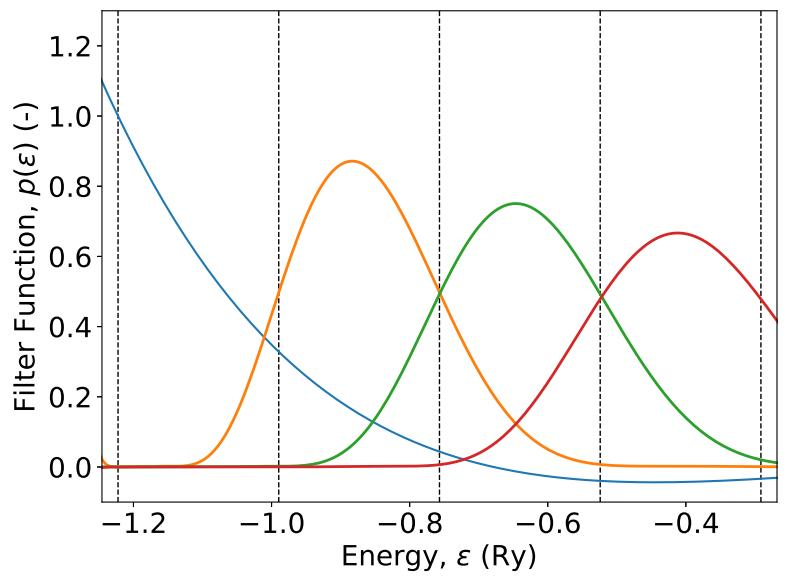
\includegraphics[keepaspectratio,alt={image}]{images/7f4d69934bd1ced88b367d01027c434c7772479c2105fa3f989f6c4920c342e3.jpg}}

Figure 6: Four filters used in the simulation of
\(\mathrm { S i _ { 1 9 4 7 } H _ { 6 0 4 } }\) . The degree of the
Chebyshev polynomial (for the leftmost slice) is 20, while the degrees
of the bandpass filters for the interior slices are 160. The dashed
lines visualize the slice bounds.

\pandocbounded{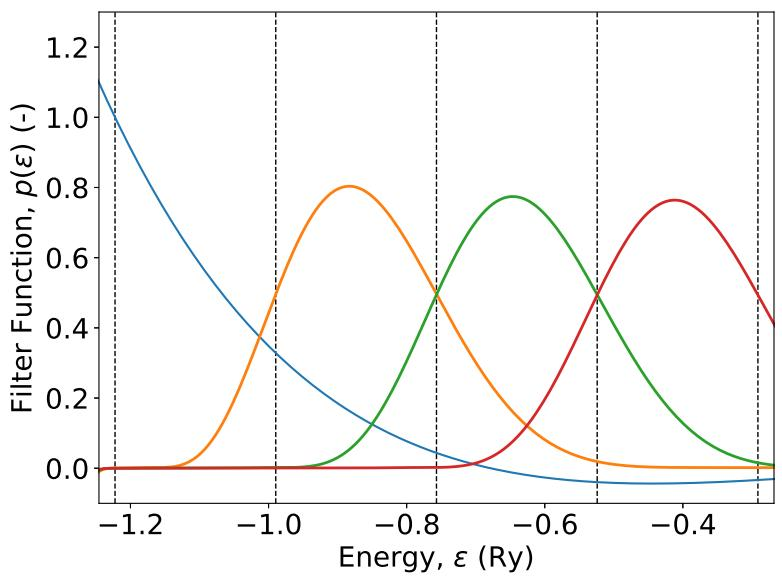
\includegraphics[keepaspectratio,alt={image}]{images/3e585f1d9f2a243356ba2dd46523213e09e26f38741ab1699d2b58c34b5ff4ad.jpg}}

Figure 7: Four filters with the same slice bounds as those in Figure 6
but of different polynomial degrees. The degree of the Chebyshev
polynomial (for the leftmost slice) is 20, while the degrees of the
bandpass filters for slices \(2 , 3 ,\) and 4 are 137, 168, and 195,
respectively. The amplifying ratio is 1.1. The dashed lines visualize
the slice bounds.

Once a partition of the spectrum into multiple slices has been
determined, the number of column groups assigned to the ith slice
\(( n _ { c _ { i } } )\) can be set according to the following formula

\[
n _ {c _ {i}} = \left\lfloor n _ {\mathrm{c}} \cdot \frac {p _ {i} m _ {i}}{\sum_ {i = 1} ^ {s} p _ {i} m _ {i}} \right\rfloor , \tag {16}
\]

where \(p _ { i }\) is the number of eigenvalues in the ith slice,
\(m _ { i }\) is the degree of the polynomial constructed for that
slice, s is the total number of slices, and \(n _ { \mathrm { c } }\) is
the total number of column groups defined in Section 4.1. Some
adjustment may be needed to ensure that
\(n _ { c _ { i } } \mathrm { ^ { * } s }\) add up to \(n _ { c } .\) .
In practice, we use a larger \(p _ { i }\) , which is the number of
eigenvalues in that slice plus some states from adjacent slices. These
extra states may originate from as many as two column groups in each of
the adjacent slices. This strategy improves the stability of the SS
algorithm and prevents the potential necessity of moving overlap states
between slices over SCF iterations.

One of the challenges in implementing SS is to choose an optimal
partition so that

\[
\max _ {i} p _ {i} m _ {i} \tag {17}
\]

is minimized. Because the degree of the Chebyshev polynomial used for
the leftmost slice is generally much lower, it makes sense to make the
leftmost slice slightly wider to include more eigenvalues. To minimize
(17), we can perform an exhaustive search on the number of slices,
\(s ,\) that yields the minimum of (17). That is, at first the degree of
the Chebyshev polynomial is set to 20. If \(2 0 p _ { 1 }\) is
significantly less than (17) for any interior slice, we merge
\(n _ { l }\) leftmost slices with \({ n _ l = 2 , 3 , . . , s - 1 }\)
until \(2 0 p _ { 1 }\) is as close to maxi \(p _ { i } m _ { i }\) as
possible.

\section{4.3. Communication}\label{communication}

There are two types of communications in both CheFSI and SS. One is
within a column group, and the other is within a slice. The
communication required in the multiplication of the Hamiltonian with a
distributed vector is limited to within each column group. Processes in
the same column group exchange data via neighborhood collective
communication. Communication overhead can be lowered by using
non-blocking communication and overlapping the communication and local
computation. Another improvement can be done is to use space-filling
curves when partitioning the real-space grid. A real-space grid
partition based on space-filling curves has good locality of neighboring
grid points and thus the communication for stencil traversal can be
reduced. This improves the efficiency and scalability of the
multiplication of H with vectors. Our preliminary result has shown that,
if not communication-bound, a speed-up of 1.5 to 2, compared with a
simple real-space grid partition, can be achieved. This will be one of
our future studies.

In CheFSI, orthonormalization of basis vectors and other dense
matrix-matrix operations such as solving the projected eigenvalue
problem involves all processes on the 2D process grid. We rely on the
communication layers implemented in PBLAS and ScaLAPACK to perform the
necessary data communication required to carry out these operations. The
communication cost can be relatively high. In SS, all dense matrix
computation is carried out among the column groups mapped to a spectral
slice. Consequently, all communication takes place within a subset of
processes, which can significantly reduce the communication overhead.

\section{5. Computational Results}\label{computational-results}

In this section, we evaluate the performance of the polynomial filtering
algorithm. The computational experiments are carried out on the Cori
Haswell compute nodes (Intel Xeon E5-2698 v3, 32 cores per node)
maintained at the National Energy Research Scientific Computing (NERSC)
Center.

We use a silicon nanocrystal with 1,947 Si atoms passivated by 604 H
atoms to test the performance of the proposed algorithm. This system is
denoted by \(\mathrm { S i _ { 1 9 4 7 } H _ { 6 0 7 } }\) below. The
finite difference order is 12, and the grid spacing is 0.7 bohr, which
corresponds to a kinetic energy cutoff of ∼20 Ry in a plane wave
representation. The simulation domain is a sphere, beyond which the wave
functions are set to zero. A margin of at least 7 bohr is preserved
between the atoms and the boundary of the simulation domain. The
Hamiltonian size is 1,527,083, and the number of states to be calculated
is set to 4,352 (though the number of occupied states is 4,196, we
include extra (unoccupied) states to accelerate the convergence, as
explained in Section 3.2.3). We use Troullier-Martins norm-conserving
pseudopotentials {[}31{]}, and for H atoms the cutoff radius for 1s is
1.80 bohr, while for Si atoms the cutoff radii for 3s/3p are 2.80/2.80
bohr, respectively. The exchange-correlation functional is local density
approximation with the parameterization by Perdew and Zunger (LDA CA PZ)
{[}32{]}. The Anderson mixing scheme {[}33{]} is used. The mixing ratio
is 0.3, and the potential mixing performed at a particular SCF iteration
uses the potentials computed in the previous 4 SCF iterations. The
convergence criterion (SRE) is set to 0.0001 Ry. Smaller silicon
nanocrystals are used to study SCF convergence with filter polynomials
of different degrees, and a larger one
\(\left( \mathrm { S i _ { 3 8 9 3 } H _ { 9 8 8 } } \right)\) is used
to study the strong parallel scalability of the SS algorithm.

In all experiments, we use CheFSI in the first few SCF iterations, and
then transition to SS in the subsequent SCF iterations. Communication
groups are created to map column groups to different spectral slices so
that the ith spectral slice owns \(n _ { c _ { i } }\) column groups,
where \(n _ { c _ { i } }\) is defined in (16). Data redistribution
among column groups is required as we transition from CheFSI to SS. Some
Ritz vectors kept on one column group are sent to adjacent column groups
to create Ritz pair overlap that can help accelerate subspace iteration
within each slice as discussed in Sections 3.2.3 and 4.2.

{\def\LTcaptype{none} % do not increment counter
\begin{longtable}[]{@{}|l|l|@{}}
\toprule\noalign{}
\endhead
\bottomrule\noalign{}
\endlastfoot
\hline
Component & Description \\
\hline
FLTR & Amplification of lowest-energy states \\
\hline
ORTH & Orthonormalization of wave functions via Cholesky QR \\
\hline
RR & Rayleigh--Ritz procedure (i.e., projection of wave functions into a
Ritz matrix, eigen-decomposition of the Ritz matrix, and subspace
rotation) \\
\hline
\end{longtable}
}

Table 1: Main computational components of subspace iteration

\section{5.1. Performance profile}\label{performance-profile}

We first report the performance characteristics of both CheFSI and SS
when they are run with 256 Cori Haswell cores. The timing measurements
of subspace iteration are grouped into the three categories listed in
Table 1.

We use a Chebyshev polynomial of degree 20 in the CheFSI calculation.
The definition of the 2D process grid for the CheFSI calculation is not
unique. For example, we can use only one column group and partition the
basis vectors into 256 row blocks, which was used in previous
implementations of the PARSEC software. At the other extreme, we can
partition the basis vectors into 256 column groups (i.e., 1 process per
column group). Figure 8 shows for one subspace iteration how the timing
measurements of different components in the CheFSI calculation change as
we change the data layout. By partitioning the basis vectors into
multiple column groups that do not require communication during
polynomial filtering (FLTR), the performance of this part can be
significantly improved. When the basis vectors are distributed among 32
columns groups (i.e., 8 process per column group), the time spent on
FLTR is reduced by a factor of 3.9 when compared with the approach in
which 256 processes are used in a single column group to perform the
multiplication of H with vectors distributed by rows among the 256
processes. However, as we continue to increase the number of column
groups and reduce the number of row blocks within each column group, the
performance of FLTR does not change much. This is because the parallel
implementation of the sparse matrix-vector multiplication Hx scales well
to a modest number of processes (in this case, 8).

However, we can also see that as the number of column groups increases,
the orthonormalizaton (ORTH) and Rayleigh--Ritz procedure (RR) in CheFSI
become more costly. This is because these components make use of
parallel dense matrix-matrix multiplication (PGEMM) which attains the
best performance with the ratio between the number of rows and the
number of columns is not too large nor small. In order to achieve
optimal performance, we use two different data layouts in the CheFSI
calculation for FLTR and other dense linear algebra computation. The
last bar in Figure 8 depicts the performance profile using a 8 × 32
process grid for FLTR, and transitioning to a 256 × 1 process grid for
other dense linear algebra operations. We use PDGEMR2D to change data
distribution. The overhead associated with data reshuffling, which is
embedded in ORTH and RR, appears to be small, as we can see from the
last bar in Figure 8.

The performance profile of the SS algorithm for one subspace iteration
is illustrated in Figure 9. The process grid is 16 × 16, and four slices
are used. The numbers of column groups in slice 1--4 are computed to be
1, 5, 6, and 4, respectively. A Chebyshev polynomial of degree 40 is
used to compute approximate eigenpairs in the leftmost slice. Bandpass
filters of degree 160 are used to compute approximate eigenpairs in the
other slices. For comparison, we also plot the performance profile using
CheFSI as the leftmost bar. The leftmost slice contains 1,334
eigenvalues among which 808 are actually within the spectral bounds
associated with that slice. Slice 2--4 contain 1,970, 2,496 and 1,820
eigenvalues, respectively. Among them 891, 1,482 and 1,015 eigenvalues
of interest are within the spectral bounds associated with these slices.
As we can see from Figure 9, FLTR takes most of the time in the SS
algorithm. All the other computational kernels (ORTH, RR) take a small
faction of the total wallclock time. Since
\(p _ { i } m _ { i } / n _ { c _ { i } }\) ≈ 64, 000, we expect the
computation to be well load-balanced as is the case. The time spent on
each slice is roughly the same (∼ 800 seconds). We can see FLTR in SS
costs about an order of magnitude more than that in CheFSI, due to the
requirement of high degree filters in SS. Though FLTR in SS is more
expensive than that in CheFSI, in this case, the cost of the cubically
scaling operations (ORTH+RR) in SS is less than that in CheFSI. This
shows the SS algorithm can indeed reduce the cost of the dense linear
algebra operations. We note that for slices 2--4 there is no time cost
shown for ORTH, because we solve a generalized eigenvalue problem for
these interior slices, so the time cost of ORTH is embedded in RR.

\pandocbounded{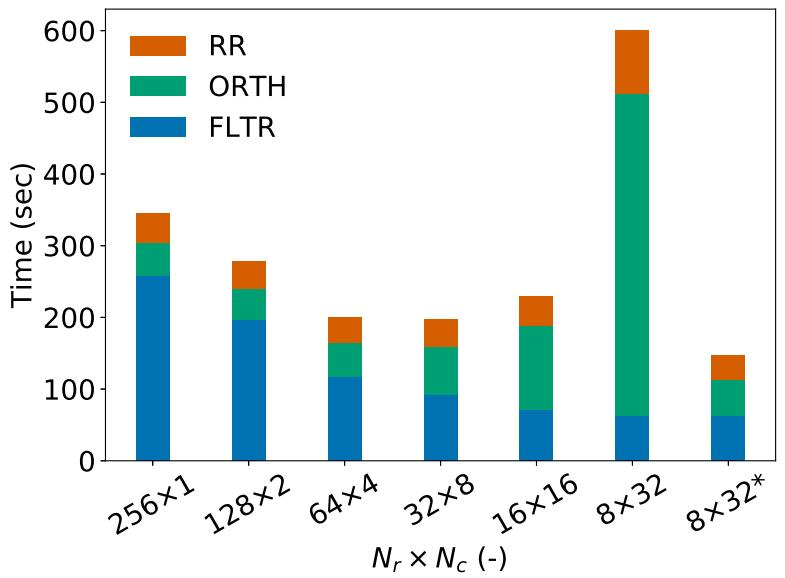
\includegraphics[keepaspectratio,alt={image}]{images/e19a7e279c0d0641ed12a6cbeb4753fdbdb9f207c16ca29536baf9b836a55688.jpg}}

Figure 8: Computational time of the key components in the CheFSI
calculations with different process grids.

Because the degrees of the bandpass filter polynomials used in SS are
much higher than the degree of the Chebyshev polynomial used in CheFSI,
we expect the wallclock time spent on FLTR to be much longer in SS than
that in CheFSI.

For this problem, the significantly higher cost of FLTR in SS cannot be
completely offset by the reduction in the cost of ORTH and RR. As a
result, the total cost of SS is still higher than that of CheFSI when
the problem is solved on 256 cores. We show in Section 5.4 that, as the
problem size becomes larger and more compute cores are used, the time
spent on ORTH and RR will start to dominate in CheFSI calculation
regardless how many compute cores are used, whereas such cost is
relatively low in SS calculation. Because FLTR can easily scale to tens
of thousands of cores, whereas it is difficult to achieve this kind of
scalability for ORTH and RR, SS will scale to much larger number of
compute cores and eventually outperform CheFSI.

\section{5.2. Comparing subspace iteration with Lanczos for spectrum
slicing}\label{comparing-subspace-iteration-with-lanczos-for-spectrum-slicing}

As we argued in Section 3.2.3, using subspace iteration to compute the
desired eigenpairs within a spectral slice has the advantage of allowing
the multiplication of H with different vectors to be performed among
different column groups on a 2D process grid. The multiple levels of
concurrency are likely to yield better parallel scalability even though
the subspace iteration method has a slower convergence rate compared
with the Lanczos algorithm, which cannot perform multiple Hamiltonian
and vector multiplications simultaneously.

Figure 10 shows, from one of the slices in the simulation of
\(\mathrm { S i _ { 1 9 4 7 } H _ { 6 0 4 } }\) , how the cumulative
wallclock time spent on both FLTR and ORTH of the Lanczos method
increases with respect to the Lanczos iteration number. We compare the
cost of the Lanczos method with that of the subspace iteration method
for a spectral slice that contains the most eigenpairs. The number of
eigenvalues in this slice is 1, 363. The degrees of the polynomials are
200. The Lanczos iteration is performed on a 1D process grid with 256
processes. The subspace iteration is carried out on a 16 × 16 2D process
grid. As expected, the wallclock time increases as we perform more
Lanczos iterations. For this slice, 2, 538 Lanczos steps are needed to
produce sufficiently accurate approximate eigenpairs. As a result, the
total number of Hamiltonian and vector multiplications used by the
Lanczos method is 2, 538 × 200 ≈ 500, 000. The corresponding wallclock
time is nearly 1, 500 seconds.

\pandocbounded{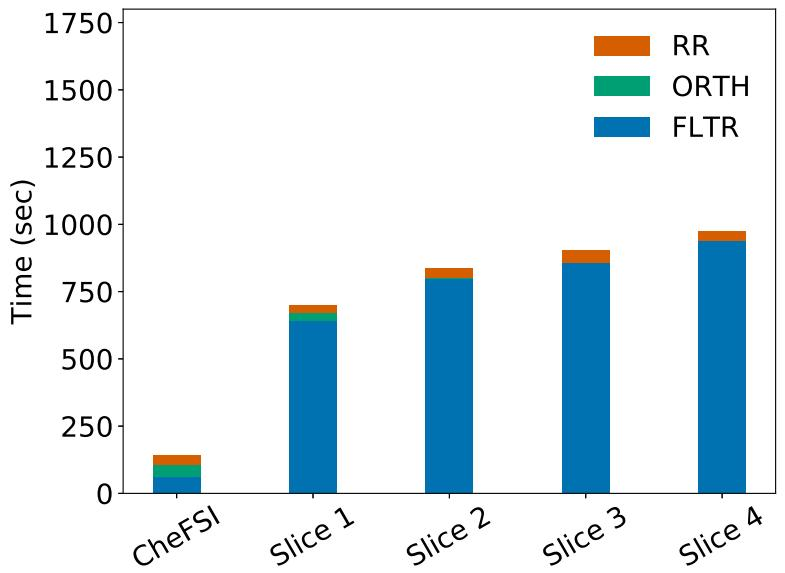
\includegraphics[keepaspectratio,alt={image}]{images/8928d14ec4b09d1b17151a8d804fd701453e37ec6dcd6115ae7b07c15d086196.jpg}}

Figure 9: Computational time of the key components in the SS
calculation. The leftmost bar shows the wallclock time by CheFSI,
serving as a reference.

When subspace iteration is used, we include 3, 616 basis vectors in the
subspace to accelerate convergence. The dashed line in Figure 10 shows
the wallclock time for one subspace iteration, which is around 700
seconds. Even though the subspace iteration perform 3, 616 × 200
\textgreater{} 720, 000 Hamiltonian and vector multiplications, which
are more than those performed in the Lanczos method, the wallclock time
used by subspace iteration is much less than that used by the Lanczos
method. This is due to the much better parallel scalability of the
subspace iteration method as we discussed earlier. We should point out
that in many cases, one subspace iteration with a sufficiently high
degree polynomial is enough to make the SCF iteration converge. However,
in some cases, more than one subspace iteration may be required to
ensure SCF convergence.

\pandocbounded{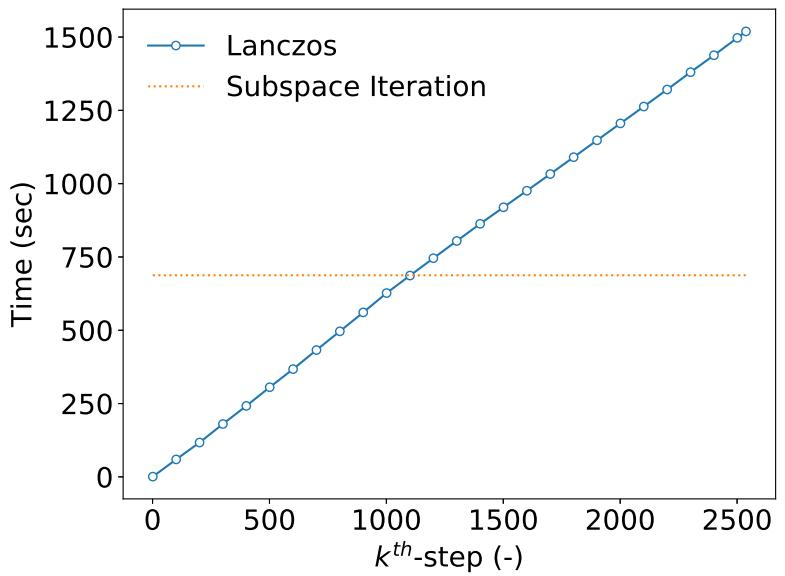
\includegraphics[keepaspectratio,alt={image}]{images/931d8c4fa6e7a1c7981308d6cedfcd272dc73380eaa8222a17e3d3f21bcd0593.jpg}}

Figure 10: Cumulative wallclock time spent on FLTR and ORTH in the
Lanczos method with respect to the Lanczos iteration number. The dashed
line shows the wallclock time using the subspace iteration method for
the same slice.

\section{5.3. SCF convergence}\label{scf-convergence}

The convergence of a SCF calculation depends partially on how well the
eigenvectors associated with occupied states and a few unoccupied states
near the Fermi level are computed. In the first few

SCF iterations, these eigenvectors do not need to be computed to full
accuracy. A few Chebyshev filtering steps starting with the eigenvectors
obtained in a previous SCF iteration are often sufficient to make the
SCF loop converge. In this section, we examine how the accuracy of the
polynomialfiltered subspace iteration method affects the convergence of
a SCF calculation. In particular, we are interested in the degrees of
the bandpass filters required in the polynomial-filtered subspace
iteration method to ensure the convergence of SCF.

We use silicon nanocrystals of different sizes for testing (the
atomistic structures of which are included as supplementary material).
These systems are listed in Table 2 along with the number of atoms,
computed states as well as the dimension of the Hamiltonians associated
with these problems. For Si29H36, only 32 compute cores are used, and we
transition from CheFSI to SS at the 2nd SCF iteration; for other cases,
256 compute cores are used, and we transition from CheFSI to SS at the
6th SCF iteration.

{\def\LTcaptype{none} % do not increment counter
\begin{longtable}[]{@{}llllllll@{}}
\toprule\noalign{}
\endhead
\bottomrule\noalign{}
\endlastfoot
\multirow{2}{*}{test problems} & \multirow{2}{*}{n} &
\multirow{2}{*}{N\_s} & \multirow{2}{*}{degree} & \multicolumn{2}{l}{%
\# of SCF iterations} & \multicolumn{2}{l@{}}{%
Time to solution} \\
& & & & CheFSI & Hybrid & CheFSI & Hybrid \\
Si\_\{29\}H\_\{36\} & 97,569 & 104 & 60 & 9 & 19 & 15 & 71 \\
Si\_\{275\}H\_\{172\} & 329,749 & 768 & 120 & 12 & 11 & 474 & 2,106 \\
Si\_\{837\}H\_\{348\} & 780,983 & 2,176 & 120 & 14 & 14 & 1,058 &
7,266 \\
Si\_\{1947\}H\_\{604\} & 1,527,083 & 4,352 & 160 & 14 & 13 & 3,070 &
35,590 \\
\end{longtable}
}

Table 2: Test problems and their sizes (in terms of the number of atoms,
the dimension of the Hamiltonian and the number of computed states), the
optimal degrees of the bandpass filter polynomials required to reach SCF
convergence, and the number of SCF iterations taken by CheFSI and SS.
The time to solution (in seconds) is compared with that of CheFSI in
which a Chebyshev polynomial of degree 20 is used.

Figure 11 shows the SCF convergence history when the hybrid CheFSI and
SS scheme is applied to Si29H36. All tests are run on a 4 × 8 process
grid. The number of column groups assigned to the three slices is (1, 4,
3). The degree of the Chebyshev polynomial is 20, and the degrees of the
bandpass filter polynomials range from 60 to 480 (Figure 11(a)). As we
can see, the SCF calculations converge in all tests. When the degrees of
bandpass filters are relatively low (e.g., 60), more SCF iterations may
be required to reach convergence. When the degrees of bandpass filters
are sufficiently high (e.g.~240 or 480), the SCF convergence history is
nearly indistinguishable from that produced by CheFSI. For this problem,
setting the degrees of bandpass filters to 60 appears to be optimal in
terms of time to solution, even though a few more SCF iterations are
required to reach convergence compared with the run in which bandpass
filters of degree 240 are used.

Due to the high degrees of the bandpass filter polynomials compared with
the Chebyshev polynomial, and also the small size of this problem for
ORTH and RR to become dominant, the time to solution of the hybrid
CheFSI-SS approach is about five times longer than that of CheFSI.

Figure 11(b) shows that it is possible to lower the degrees of bandpass
filters to 60 at the expense of performing a few subspace iterations in
one SCF iteration. Among all the tests, it appears that performing one
subspace iteration per SCF iteration yields the shortest time to
solution. Moreover, instead of performing a fixed number of subspace
iterations, we can terminate subspace iterations by checking the
residual norms of the approximate eigenpairs as discussed in Section
3.2.4. However, in this case, it appears that such a termination
criterion (which we label as ``dynamic'') is too stringent.

We can see from Table 2 that high degree bandpass filters are possibly
needed as the problem size increases, although the increase in degree is
modest. For the larger problem Si1947H604, the optimal degree appears to
be 160 instead of 120 (Figure 12). In Figure 12 the degrees of the
bandpass filters are 120, 160, and 200. The number of subspace
iterations is dynamic. In our implementation, during a SCF iteration we
run subspace iterations until either a maximum number of subspace
iterations is reached or until the relative residual norms of all
desired eigenpairs are sufficiently small (10−2 in our simulations).
This is why the time to solution is less when the degree is set to 160,
compared with the run using degree 120. In both runs, the total number
of SCF iterations required to reach convergence is almost the same. The
distribution of the occupied states and the slice bounds are included as
supplementary material.

\section{5.4. Parallel scalability}\label{parallel-scalability}

We now examine the strong parallel scalability of the SS algorithm and
compare it with that of CheFSI. We use a
\(\mathrm { S i _ { 3 8 9 3 } H _ { 9 8 8 } }\) silicon nanocrystal for
this test. The dimension of the Hamiltonian is 2, 637, 711. The number
of states to be computed is 9, 216. Both the CheFSI and SS calculation
are performed on 2D process grids with \(n _ { r } \times n _ { c }\)
processes. Our strong scaling tests use 256, 512, 1,024, 2,048, and
4,096 compute cores. In all tests, \(n _ { r }\) is set to 32. For
CheFSI, we try \(n _ { c } = 8 , 1 6 , 3 2 , 6 4\) , and 128. For SS,
the spectrum is divided into 2, 4, 8, and 16 slices. The number of
column groups for each slice is (1, 15), (1, 9, 13, 9), (1, 9, 6, 9, 8,
14, 10, 7), and (1, 6, 9, 8, 5, 6, 10, 7, 6, 10, 12, 14, 12, 7, 4, 11),
respectively. The degree of the Chebyshev polynomial is 20, and the
degrees of the bandpass filter polynomials are 120.

\pandocbounded{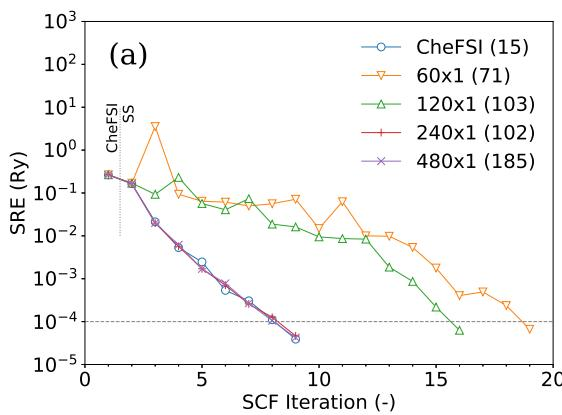
\includegraphics[keepaspectratio,alt={image}]{images/dc77e6789b7eaf53ed0842b88b310f5e01383fd34f59365ef9d6cb2b5f4c991e.jpg}}

\pandocbounded{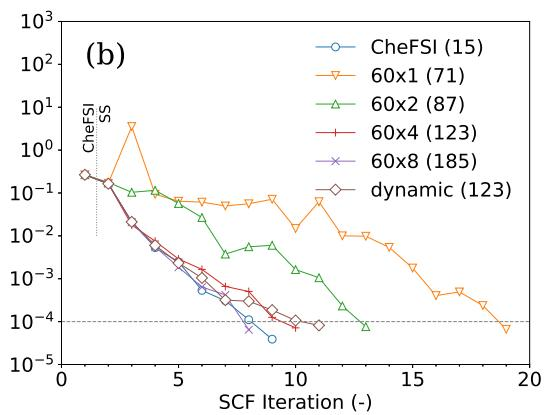
\includegraphics[keepaspectratio,alt={image}]{images/38f7ade7dd1c45bb5d6d39b62f366676c1e704d04ec23ec57cd0490dccb8f3b5.jpg}}

Figure 11: Convergence history of the simulations of Si29H36. In (a),
bandpass filter polynomials of different degrees are used, and the
number of subspace iterations per SCF iteration is one. In (b), we fix
the polynomial degree and vary the number of subspace iterations per SCF
iteration. The time to solution in seconds is shown in parentheses.

\pandocbounded{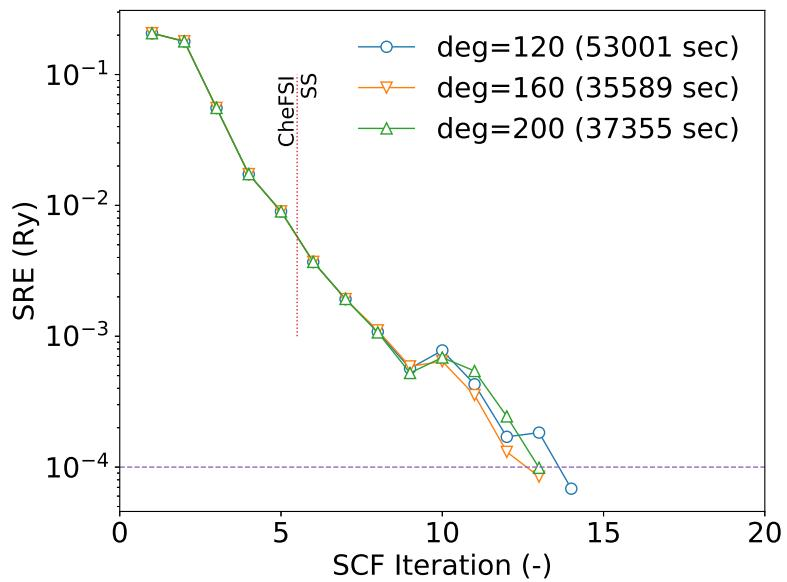
\includegraphics[keepaspectratio,alt={image}]{images/a4c16ccd73e4b6a93b963d5450a952480e94777bf66265a34483cca21c4a9739.jpg}}

Figure 12: Convergence history of the simulations of Si1947H604. The
time to solution is shown in parentheses.

We can clearly see from Figure 13 that FLTR in both CheFSI and SS has
nearly perfect parallel scalability. The cost of FLTR in SS is ∼ 5 times
of that associated with CheFSI owing to the higher degree of the
bandpass filter polynomials. We also note that due to the large number
of states to be included in the SCF calculation, ORTH and RR in CheFSI
take more time than FLTR which consists of mostly sparse matrix vector
multiplications.

By dividing the spectrum into more slices, the cost of ORTH and RR can
be significantly reduced through a trivial parallelization at the slice
level. Because ORTH and RR are performed among fewer column groups and
uses fewer processes, good scalability can be achieved in these
calculations. This can be seen from the green curve marked by empty
circles in Figure 13. The scalabilty of these types of operations is
harder to achieve in CheFSI when many column groups must be distributed
on many processes. The green curve marked by solid circles shows the
cost of ORTH and RR in CheFSI actually increases when \(n _ { c }\)
becomes larger than 16.

As a result, the overall strong scalability of SS is much better than
that of CheFSI. When the

total number of processes reaches 32×64, the computational time of SS is
less than that of CheFSI.

We should note that more states are computed in SS and the overall
subspace size in SS is larger than that in CheFSI, because the subspace
for each slice is augmented in order to improve convergence and avoid
missing states (see Section 4.2). However, because SS is compute-bound
in comparison with CheFSI which is communication-bound (due to the
communication overhead when performing ORTH and RR among all states), it
is likely to outperform CheFSI if the degrees of bandpass filter
polynomials are not too high and the number of subspace iterations is
moderate.

\pandocbounded{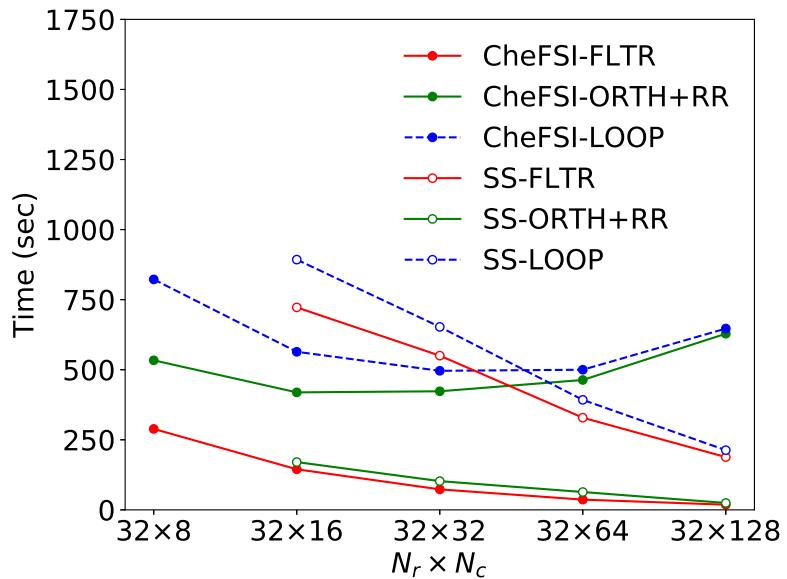
\includegraphics[keepaspectratio,alt={image}]{images/67228ff4e8ad8c74ae456674026290b720d981b9914cb5df73c8b85967e05e7e.jpg}}

Figure 13: Strong scaling test of Si3893H988. ``LOOP'' is the sum of all
operations. The computational time shown here is for one subspace
iteration.

\section{6. Conclusion}\label{conclusion}

The work described in this paper extends the spectrum slicing framework
established in the work of Schofield et al.~{[}26{]}. We discussed
several practical issues in implementing polynomial filtering for
solving the Kohn--Sham DFT problem in real space. We proposed using a
hybrid Chebyshev and bandpass filter polynomial filtering scheme to
compute the invariant subspace required to construct the electronic
charge density. The latter type of polynomial filtering is combined with
the spectrum slicing method {[}26{]} designed to reduce the
computational overhead involved in solving the projected eigenvalue
problem in the CheFSI method. We showed how to partition the spectrum
based on an estimated density of states that can be obtained from a few
Lanczos iterations. We proposed using subspace iteration (instead of
thick-restarted Lanczos iteration) to compute approximate eigenpairs
within each interior spectral slice in the spectrum slicing algorithm.
Harmonic Ritz vectors (instead of Ritz vectors) are used as approximate
eigenvectors. To achieve scalable parallel performance, we used a 2D
process grid that allows the multiplication of H with multiple vectors
to be performed efficiently. We discussed how to partition and map
column groups within the 2D process grid to spectrum slices to achieve
good load balance in the spectrum slicing procedure. Numerical examples
were presented to show the the performance profiles of both the CheFSI
and SS components of the computation.

We also showed that the use of SS does not affect the convergence of SCF
calculation provided the degree of the filtering polynomial is
sufficiently high or a sufficient number of subspace iterations is
taken. We demonstrated that for large problems SS can outperform CheFSI
on a large number of compute cores due to the higher level concurrency
of the algorithm and reduced cost for solving the projected subspace
problem, despite the much larger number of Hamiltonian vector
multiplications used by the algorithm. The optimal performance of the SS
algorithm depends largely on how the spectrum is partitioned and how
computational resources are allocated to different spectrum slices. This
is currently done in a case by case manner. An efficient procedure can
be developed to automate this process.

We should also note that a number of techniques such as the use of mixed
precision arithmetic to reduce data movement and memory requirement and
overlapping computation and communication can be used to further improve
the performance of both CheFSI and SS for large-scale simulations
performed on next-generation supercomputers that are equipped with
accelerators. These techniques have been demonstrated to be effective by
Das et al.~{[}34{]}. We will adopt some of these techniques in our
future work.

\section{7. Acknowledgments}\label{acknowledgments}

C.Y. is supported by the Center for Computational Study of Excited-State
Phenomena in Energy Materials (C2SEPEM) at LBNL, which is funded by the
U.S. DOE, Office of Science, Basic Energy Sciences, Materials Sciences
and Engineering Division under Contract No.~DE-AC02-05CH11231, as part
of the Computational Materials Sciences Program. K.-H.L. and J.R.C. are
supported by the same under a subcontract. Computational resources are
provided by the National Energy Research Scientific Computing Center
(NERSC).

\section{References}\label{references}

{[}1{]} P. Hohenberg, W. Kohn, Inhomogeneous electron gas, Phys.
Rev.~136 (3B) (1964) B864--B871. doi:10.1103/PhysRev.136.B864. URL
https://link.aps.org/doi/10.1103/PhysRev.136.B864

{[}2{]} W. Kohn, L. J. Sham, Self-consistent equations including
exchange and correlation effects, Phys. Rev.~140 (4A) (1965)
A1133--A1138. doi:10.1103/PhysRev.140.A1133. URL
https://link.aps.org/doi/10.1103/PhysRev.140.A1133

{[}3{]} K.-H. Liou, J. R. Chelikowsky (to be published.).

{[}4{]} Y. Zhou, Y. Saad, M. L. Tiago, J. R. Chelikowsky, Parallel
self-consistent-field calculations via Chebyshev-filtered subspace
acceleration, Phys. Rev.~E 74 (6) (2006) 066704. doi:10.
1103/PhysRevE.74.066704. URL
https://link.aps.org/doi/10.1103/PhysRevE.74.066704

{[}5{]} Y. Zhou, J. R. Chelikowsky, Y. Saad, Chebyshev-filtered subspace
iteration method free of sparse diagonalization for solving the
Kohn--Sham equation, J. Comput. Phys. 274 (2014) 770--782.
doi:10.1016/j.jcp.2014.06.056. URL
http://www.sciencedirect.com/science/article/pii/S0021999114004744

{[}6{]} J. R. Chelikowsky, M. L. Tiago, Y. Saad, Y. Zhou, Algorithms for
the evolution of electronic properties in nanocrystals, Comput. Phys.
Commun. 177 (1) (2007) 1--5. doi:10.1016/j. cpc.2007.02.072. URL
http://www.sciencedirect.com/science/article/pii/S0010465507000458

{[}7{]} W. Hu, L. Lin, C. Yang, DGDFT: A massively parallel method for
large scale density functional theory calculations, J. Chem. Phys. 143
(12) (2015) 124110. doi:10.1063/1.4931732. URL
https://aip.scitation.org/doi/abs/10.1063/1.4931732

{[}8{]} S. Ghosh, P. Suryanarayana, SPARC: Accurate and efficient
finite-difference formulation and parallel implementation of density
functional theory: Isolated clusters, Comput. Phys. Commun. 212 (2017)
189--204. doi:10.1016/j.cpc.2016.09.020. URL
http://www.sciencedirect.com/science/article/pii/S0010465516303046

{[}9{]} B. Kanungo, V. Gavini, Large-scale all-electron density
functional theory calculations using an enriched finite-element basis,
Phys. Rev.~B 95 (3) (2017) 035112. doi:10.1103/PhysRevB. 95.035112. URL
https://link.aps.org/doi/10.1103/PhysRevB.95.035112

{[}10{]} J. Winkelmann, P. Springer, E. D. Napoli, ChASE: Chebyshev
accelerated subspace iteration eigensolver for sequences of hermitian
eigenvalue problems, ACM Trans. Math. Softw. 45 (2) (2019) 21:1--21:34.
doi:10.1145/3313828. URL http://doi.acm.org/10.1145/3313828

{[}11{]} V. Michaud-Rioux, L. Zhang, H. Guo, RESCU: A real space
electronic structure method, J. Comput. Phys. 307 (2016) 593--613.
doi:10.1016/j.jcp.2015.12.014. URL
http://www.sciencedirect.com/science/article/pii/S0021999115008335

{[}12{]} A. S. Banerjee, L. Lin, P. Suryanarayana, C. Yang, J. E. Pask,
Two-level Chebyshev filter based complementary subspace method: Pushing
the envelope of large-scale electronic structure calculations, J. Chem.
Theory Comput. 14 (6) (2018) 2930--2946. doi:10.1021/acs.jctc. 7b01243.
URL https://doi.org/10.1021/acs.jctc.7b01243

{[}13{]} J. Chelikowsky, Introductory Quantum Mechanics with MATLAB: For
Atoms, Molecules, Clusters, and Nanocrystals, Wiley, 2019.

{[}14{]} L. Kronik, A. Makmal, M. L. Tiago, M. M. G. Alemany, M. Jain,
X. Huang, Y. Saad, J. R. Chelikowsky, PARSEC -- the pseudopotential
algorithm for real-space electronic structure calculations: recent
advances and novel applications to nano-structures, Phys. Stat. Sol. (b)
243 (5) (2006) 1063--1079. doi:10.1002/pssb.200541463. URL
https://onlinelibrary.wiley.com/doi/abs/10.1002/pssb.200541463

{[}15{]} R. Li, Y. Xi, E. Vecharynski, C. Yang, Y. Saad, A thick-restart
Lanczos algorithm with polynomial filtering for hermitian eigenvalue
problems, SIAM J. Sci. Comput. 38 (4) (2016) A2512--A2534.
doi:10.1137/15M1054493. URL
https://epubs.siam.org/doi/abs/10.1137/15M1054493

{[}16{]} R. Lehoucq, D. Sorensen, C. Yang, ARPACK Users' Guide, Society
for Industrial and Applied Mathematics, 1998.
doi:10.1137/1.9780898719628. URL
https://epubs.siam.org/doi/abs/10.1137/1.9780898719628

{[}17{]} A. V. Knyazev, Toward the optimal preconditioned eigensolver:
Locally optimal block preconditioned conjugate gradient method, SIAM J.
Sci. Comput. 23 (2) (2001) 517--541. doi:10.1137/S1064827500366124. URL
https://epubs.siam.org/doi/abs/10.1137/S1064827500366124

{[}18{]} E. R. Davidson, The iterative calculation of a few of the
lowest eigenvalues and corresponding eigenvectors of large
real-symmetric matrices, J. Comput. Phys. 17 (1) (1975) 87--94. doi:
10.1016/0021-9991(75)90065-0. URL
http://www.sciencedirect.com/science/article/pii/0021999175900650

{[}19{]} J. A. Duersch, M. Y. Shao, C. Yang, M. Gu, A robust and
efficient implementation of LOBPCG, SIAM J. Sci. Comput. 40 (5) (2018)
C655--C676. doi:10.1137/17M1129830. URL
https://epubs.siam.org/doi/abs/10.1137/17M1129830

{[}20{]} E. L. Stiefel, Kernel polynomials in linear algebra and their
numerical applications, Nat. Bur. Standards Appl. Math. Ser. 49 (1958)
1--22.

{[}21{]} C. Yang, Accelerating the Arnoldi iteration -- theory and
practice, Ph.D.~thesis, Rice University, Houston, TX (1998).

{[}22{]} Y. Zhou, Y. Saad, M. L. Tiago, J. R. Chelikowsky,
Self-consistent-field calculations using Chebyshev-filtered subspace
iteration, J. Comput. Phys. 219 (1) (2006) 172--184. doi:10.
1016/j.jcp.2006.03.017. URL
http://www.sciencedirect.com/science/article/pii/S002199910600146X

{[}23{]} B. Parlett, The Symmetric Eigenvalue Problem, Society for
Industrial and Applied Mathematics, 1998. doi:10.1137/1.9781611971163.
URL https://epubs.siam.org/doi/abs/10.1137/1.9781611971163

{[}24{]} G. H. Golub, C. F. V. Loan, Matrix Computations (3rd Ed.),
Johns Hopkins University Press, 1996.

{[}25{]} Y. Saad, Chebyshev acceleration techniques for solving
nonsymmetric eigenvalue problems, Math. Comp. 42 (1984) 567--588.
doi:10.1090/S0025-5718-1984-0736453-8. URL
https://www.ams.org/journals/mcom/1984-42-166/S0025-5718-1984-0736453-8/

{[}26{]} G. Schofield, J. R. Chelikowsky, Y. Saad, A spectrum slicing
method for the Kohn--Sham problem, Comput. Phys. Commun. 183 (3) (2012)
497--505. doi:10.1016/j.cpc.2011.11. 005. URL
http://www.sciencedirect.com/science/article/pii/S0010465511003675

{[}27{]} L. Lin, Y. Saad, C. Yang, Approximating spectral densities of
large matrices, SIAM Rev.~58 (1) (2016) 34--65. doi:10.1137/130934283.
URL https://epubs.siam.org/doi/abs/10.1137/130934283

{[}28{]} L. Trefethen, D. Bau, Numerical Linear Algebra, Society for
Industrial and Applied Mathematics, 1997.

{[}29{]} G. Stewart, Matrix Algorithms, Society for Industrial and
Applied Mathematics, 2001. doi: 10.1137/1.9780898718058. URL
https://epubs.siam.org/doi/abs/10.1137/1.9780898718058

{[}30{]} G. L. Sleijpen, J. v. d.~Eshof, On the use of harmonic Ritz
pairs in approximating internal eigenpairs, Linear Algebra Appl. 358 (1)
(2003) 115--137. doi:10.1016/S0024-3795(01) 00480-3. URL
http://www.sciencedirect.com/science/article/pii/S0024379501004803

{[}31{]} N. Troullier, J. L. Martins, Efficient pseudopotentials for
plane-wave calculations, Phys. Rev.~B 43 (3) (1991) 1993--2006.
doi:10.1103/PhysRevB.43.1993. URL
https://link.aps.org/doi/10.1103/PhysRevB.43.1993

{[}32{]} J. P. Perdew, A. Zunger, Self-interaction correction to
density-functional approximations for many-electron systems, Phys.
Rev.~B 23 (10) (1981) 5048--5079. doi:10.1103/PhysRevB.23. 5048. URL
https://link.aps.org/doi/10.1103/PhysRevB.23.5048

{[}33{]} V. Eyert, A comparative study on methods for convergence
acceleration of iterative vector sequences, J. Comput. Phys. 124 (2)
(1996) 271--285. doi:10.1006/jcph.1996.0059. URL
http://www.sciencedirect.com/science/article/pii/S0021999196900595

{[}34{]} S. Das, P. Motamarri, V. Gavini, B. Turcksin, Y. W. Li, B.
Leback, Fast, scalable and accurate finite-element based ab initio
calculations using mixed precision computing: 46 pflops simulation of a
metallic dislocation system, in: Proceedings of the International
Conference for High Performance Computing, Networking, Storage and
Analysis, SC '19, Association for Computing Machinery, New York, NY,
USA, 2019. doi:10.1145/3295500.3357157. URL
https://dl.acm.org/doi/10.1145/3295500.3357157

\end{document}
